\documentclass[12pt]{spieman}  % 12pt font required by SPIE;
%\documentclass[a4paper,12pt]{spieman}  % use this instead for A4 paper
\usepackage{amsmath,amsfonts,amssymb}
\usepackage{graphicx}
\usepackage{setspace}
\usepackage{tocloft}
\usepackage{lineno}

\newcommand{\electron}{$\text{e}^-$}

% \renewcommand{\baselinestretch}{1.65} % Change to 1.65 for double spacing

\title{Modeling and performance analysis of Implicit Electric Field Conjugation with two deformable mirrors applied to the Roman Coronagraph}

\author[a]{Kian Milani}
\author[b]{Ewan S. Douglas}
\author[b]{Sebastiaan Y. Haffert}
\author[b]{Kyle Van Gorkom}
\affil[a]{University of Arizona, Wyant College of Optical Sciences, Tucson, Arizona, United States}
\affil[b]{University of Arizona, Steward Observatory, Tucson, Arizona, United States}

\linenumbers

\renewcommand{\cftdotsep}{\cftnodots}
\cftpagenumbersoff{figure}
\cftpagenumbersoff{table} 
\begin{document} 
\maketitle

\begin{abstract}
High-order wavefront sensing and control (HOWFSC) of phase and amplitude is key to create a dark hole region within the coronagraphic image plane where high contrasts are achieved. The Roman Coronagraph is expected to perform its HOWFSC with a ground-in-the-loop scheme due to the computational complexity of the Electric Field Conjugation (EFC) algorithm. This scheme provides the flexibility to alter the HOWFSC algorithm for given science objectives. The baseline HOWFSC scheme involves running EFC while observing a bright star such as $\zeta$ Puppis to create the initial dark hole followed by a slew to the science target.

The new implicit EFC (iEFC) algorithm removes the optical diffraction model from the controller, making the final contrast independent of model accuracy. While previously demonstrated with a single DM, iEFC is extended to two deformable mirror systems in order to create annular dark holes. First, an overview of both EFC and iEFC is presented. The algorithm is then applied to the Wide-Field-of-View Shaped Pupil Coronagraph mode designed for the Roman Space Telescope using end-to-end physical optics models. Initial noiseless monochromatic simulations demonstrate the efficacy of iEFC as well as the optimal choice of modes for the SPC-WFOV instrument. Further simulations for the 3.6\% wavefront control bandpass with noise yield estimation times for calibration and subsequent contrast results where the reference star used for iEFC is assumed to be $\zeta$ Puppis. Contrasts comparable to EFC are achieved: approximately $2\times10^{-9}$ for noiseless monochromatic simulations while the broadband simulations with noise converge to contrasts of $10^{-8}$. The estimated time to measure the iEFC Jacobian is 27 hours; however, a discussion is provided for how this calibration time could be reduced. The results here indicate that iEFC can be a valid HOWFSC method that can mitigate the risk associated with space-borne coronagraphs.
% Suppressing speckles in a dark hole region of a coronagraph image plane via high-order wavefront sensing and control (HOWFSC) of phase and amplitude is key to directly imaging planets in reflected light. The Roman Coronagraph is expected to perform its HOWFSC with a ground-in-the-loop scheme due to the computational complexity of the Electric Field Conjugation (EFC) algorithm. This scheme provides the flexibility to alter the HOWFSC algorithm for given science objectives. The baseline HOWFSC scheme involves running EFC while observing a bright star such as $\zeta$ Puppis to create the initial dark hole followed by a slew to the science target while maintaining the contrast with low-order WFSC during the science observation. 

% The new implicit EFC (iEFC) algorithm removes the optical diffraction model from the controller, making the final contrast independent of model accuracy. While previously demonstrated with a single DM, iEFC is extended to two deformable mirror systems in order to create annular dark holes. An overview of both EFC and iEFC is presented to clarify the principle of iEFC and how the modal coefficients for two DMs are found. The algorithm is then applied to the Wide-Field-of-View Shaped Pupil Coronagraph mode designed for the Roman Space Telescope using end-to-end physical optics models based on the PROPER models. Initial noiseless monochromatic simulations demonstrate the efficacy of iEFC as well as the optimal choice of modes for the SPC-WFOV instrument. Further simulations for the 3.6\% wavefront control bandpass with noise yield estimation times for calibration and subsequent contrast results where the reference star used for iEFC is assumed to be $\zeta$ Puppis. Contrasts comparable to EFC are achieved: approximately $2\times10^{-9}$ for noiseless monochromatic simulations while the broadband simulations with noise converge to contrasts of $10^{-8}$ with a single calibration of iEFC. The estimated time to measure the iEFC Jacobian is 27 hours; however, a discussion is provided for how this calibration time could be reduced. The results here indicate that iEFC can be a valid HOWFSC method that can mitigate the risk associated with space-borne coronagraphs that cannot be serviced. 
\end{abstract}

% Include a list of up to six keywords after the abstract
\keywords{coronagraph, dark hole, deformable mirrors, contrast}

% Include email contact information for corresponding author
{\noindent \footnotesize\textbf{*}Kian Milani,  \linkable{kianmilani@arizona.edu} }

\begin{spacing}{2}   % use double spacing for rest of manuscript

\section{Introduction}
\label{sec:intro}
With thousands of exoplanets having been discovered primarily via indirect detection methods including transit photometry and radial velocity measurements, further studies are desired to understand the dynamics of planet formation, interactions with debris disks, and aid the discovery of potentially habitable worlds. These studies can be enabled if the challenges of direct-imaging are overcome, of which the two primary challenges are the relatively small angular separation between the host star and the exoplanet as well as the small planet to star flux ratio. For perspective, a Sun-Earth analog at 10 parsecs will have an angular separation of about 0.1 arcsec and a flux ratio of about $10^{-10}$\cite{woolf-earth-like-contrast-1998}. While coronagraphs and high-order wavefront control algorithms have been demonstrated under laboratory conditions with ground-based instruments \cite{potier-vlt-sphere-efc}\cite{ahn-combining-efc-ldfc}, atmospheric turbulence, telescope stability, and absorption in certain bandpasses limit ground-based performance. A key milestone for direct-imaging will be the launch of the Nancy Grace Roman Space Telescope, which will carry an onboard coronagraph with multiple modes for imaging and spectral characterization\cite{noecker-wfirst-afta-2016}. 

While acting as a technology demonstration, the Roman Coronagraph is expected to bridge the performance gap between current high-contrast imaging capabilities and what is expected for a future 6 meter class Habitable Worlds Observatory (HWO) recommended by the decadal survey to image Earth-like exoplanets\cite{astro2020decadal}. Predicted to achieve contrasts on the order of $10^{-9}$,\cite{Bailey-roman-cgi-2023} the Coronagraph Instrument is particularly focused on demonstrating two distinct coronagraph designs, low-noise electron multiplying detectors, and high-order wavefront sensing and control (HOWFSC) algorithms required to suppress speckles from static aberrations within the optical train. The primary method intended for the HOWFSC scheme has been the use of model-based Electric Field Conjugation (EFC)\cite{give'on-bb-wavefront-correction}. Described in Section \ref{sec:efc}, EFC is combined with Pairwise Probing (PWP) in order to sense and minimize the focal plane electric field using an instrument model. Currently, EFC is expected to achieve the desired contrasts for Roman. However, EFC performance has been demonstrated to degrade by an order of magnitude in contrast due to inaccuracies in the model, particularly those associated with the DM actuators\cite{potier-comparing-fpwfs}. This is the motivation to study the alternative implicit EFC method \cite{haffert-iefc} where the Jacobian is constructed entirely from empirical data which includes all perturbations in the optical system. For a space-borne telescope, iEFC can be a particularly valuable method as it can mitigate the risk associated with instrument performance in the presence of instrument uncertainties. In addition, iEFC does not require the focal plane electric field to be sensed prior to computing the actuator commands, simplifying the algorithm as fewer parameters need to be optimized within the iEFC controller\cite{haffert-iefc}.

Here, iEFC is extended to use 2 DMs and proven capable of creating an annular dark hole such that it can be applied to the Roman Coronagraph as well as designs for future missions such the HWO. The SPC-WFOV mode is chosen because preliminary simulations demonstrated that iEFC is likely not suited to the Hybrid Lyot Coronagraph (HLC) due to the frequent relinearization of the Jacobian required for the HLC if the DM design patterns are not used\cite{milani-cgi-iefc-2023} or used slightly incorrectly\cite{zhou-cgi-howfsc-2020}. Specifically, the empirical calibration of the iEFC Jacobian would make repeated relinearizations unfeasible for the Coronagraph because of the required duration of each Jacobian calibration. %particularly because improvements in contrast would then require longer exposure times during the next calibration.

Section \ref{sec:iefc} provides a brief overview of the iEFC algorithm as well as a simple demonstration using two DMs with a scalar vortex coronagraph (SVC). This is followed by demonstration of EFC for the SPC-WFOV mode that illustrates how instrument perturbations unaccounted for in a model result in degraded performance of EFC. The efficacy of iEFC is simulated for Roman using monochromatic simulations in Section \ref{sec:mono-iefc} where iEFC is simulated using multiple modal basis to demonstrate which is optimal for the SPC-WFOV instrument. Additional results for broadband simulations that include noise are presented in Section \ref{sec:bb-iefc}, where the optimal modal basis from the monochromatic simulations are used. The choice of probes is also discussed in order to mitigate the effects of noise during the calibration of iEFC. The end-to-end model used for all SPC-WFOV simulations are described in Section \ref{sec:roman-pom}. The results demonstrate that iEFC is a suitable method for the SPC-WFOV mode and can mitigate the risk of pupil misalignments after the launch of Roman, but the calibration times required demonstrate why iEFC has further potential for future missions with larger apertures for photon collection. 

\section{Definitions and Algorithm}
\label{sec:defs}
All variables will contain subscripts to describe the quantity the variable represents. Scalars, matrices, and operators are represented by variables with standard font while variables in bold font represent column vectors. Most images presented will be in units of normalized intensity (NI), defined as $$I_N = I_{image}(x,y)/max(I_{uo}(x,y))$$ where $I_{image}(x,y)$ is the intensity of a raw coronagraphic image and $I_{uo}(x,y)$ is the intensity of an unocculted PSF (no focal plane mask in the optical train). While not a direct measurement of contrast, this metric is closely related and is the same used in FALCO\cite{sidick-falco-2}. When contrast is referenced in latter sections, it will refer to this definition of normalized intensity. 

\subsection{EFC}
\label{sec:efc}
Following the formalism of EFC from Give'on et al.\cite{give'on-bb-wavefront-correction}, the fundamental concept of EFC is that the irradiance in the image plane can be minimized by computing DM commands that destructively interfere with the measured electric field\cite{give'on-bb-wavefront-correction}. This is done by using a model of the instrument to estimate the influence of DM modes on the electric field in the image plane. For a coronagraph, this electric field may be written as some linear operation $C[\text{\space}]$ acting on the pupil plane wavefront $Ae^{\alpha + i\beta}$ where $A$ is a constant amplitude, $\alpha$ is the parameter corresponding to amplitude aberrations, and $\beta$ is the parameter corresponding to phase aberrations.

\begin{equation}
    \label{eq:efc-1}
    E_{im} = C[Ae^{\alpha + i\beta}]
\end{equation}

With coronagraphs comprising multiple relays between pupil planes and focal planes, $C[\text{\space}]$ is often a series of Fourier Transforms propagating the wavefront between the transverse planes. For a system with a single DM, the electric field can be written as 

\begin{equation}
    \label{eq:efc-2}
    E_{im} = C[Ae^{\alpha + i\beta}e^{i\phi_{DM}}]\text{.}
\end{equation}

\noindent Here, $\phi_{DM}$ is the phase induced by the surface of the DM expressed as a sum of weighted influence functions with the expression \begin{equation}
    \phi_{DM} = \frac{4\pi}{\lambda}\sum_{n=1}^{N_{acts}} a_n F_n\text{.} 
\end{equation} Assuming that the DM surface imparts a small phase, the DM phasor can be approximated as $e^{i\phi_{DM}} \approx 1 + i\phi_{DM}$, allowing for the following simplification to the image plane electric field.

\begin{equation}
    \label{eq:efc-3}
    E_{im} = C[Ae^{\alpha + i\beta}] + iC[A\phi_{DM}]
\end{equation}

Now sampled by the science camera detector,  $E_{im}$ is written as the concatenated vector $\mathbf{E_{im}}$ containing the real and imaginary components of the electric field at each pixel in the dark hole. The individual terms for the electric field contributed by the system aberrations and the DM influence functions are now written as $C[Ae^{\alpha + i\beta}] = \mathbf{E_{ab}}$ and $iC[A\phi_{DM}] = G\mathbf{A}$ respectively. Typically, $G$ is a Jacobian that transforms the actuator heights $\mathbf{A}$ into the electric field contributed by the DM at the focal plane. Here, this is written more generally as $G\mathbf{m_c}$ where $\mathbf{m_c}$ is the vector of modal coefficients for the modes calibrated. With this, the image plane electric field is written as a system of linear equations. 

\begin{equation}
    \label{eq:efc-3}
    \mathbf{E_{im}} = \mathbf{E_{ab}} + G \mathbf{m_c}
\end{equation}

As presented in Will et al.\cite{will-adefc-2021}, when a second DM is used outside a pupil plane, this system of linear equations is expanded to include the term $G_2 \mathbf{m_{c2}}$. While similar to the Jacobian for the pupil plane DM, the Jacobian $G_2$ includes the angular spectrum propagation affects from the plane of the second DM back to the pupil plane. As a system of linear equations, the two Jacobians can be concatenated to capture the influence of all DM modes such that the final equation for the image plane electric field is simplified to

\begin{equation}
    \label{eq:efc-3}
    \begin{split}
    \mathbf{E_{im}} = \mathbf{E_{ab}} + G_1 \mathbf{m_{c1}} + G_2 \mathbf{m_{c2}} = \mathbf{E_{ab}} + G_{12} \mathbf{m_{c12}} 
    \\
    \text{where } G_{12} = [G_1, G_2] \text{ and } \mathbf{m_{c12}} = \begin{bmatrix}\mathbf{m_{c1}} \\\mathbf{m_{c2}}\end{bmatrix}
    \end{split}
\end{equation}

Figure \ref{fig:efc-flowchart} illustrates the typical practices for how EFC is calibrated and performed. In EFC, the solution for modal coefficients to minimize the electric field are commonly found by minimizing a cost function such as 
\begin{equation}
    J = |\mathbf{E_{ab}} + G_{EFC}\mathbf{m_c}|^2  + \lambda|\mathbf{m_c}|^2
\end{equation}
\noindent where $\lambda$ is a regularization parameter penalizing the use of large actuator strokes. In practice, many regularization terms can be used for a variety of applications. For example, the simulations in Sections \ref{sec:mono-iefc} and \ref{sec:bb-iefc} include a weighted least squares regularization where the pixels within the control region are weighted to target specific regions of the dark hole. Once the regularization method is chosen, the pseudo-inverse of $G_{EFC}$ is computed to get the control matrix $M_C$. The modal coefficients that minimize the cost function are calculated with the matrix-vector product $M_C\mathbf{E_{ab}}$. The matrix $M_{modes}$ contains each of the modes calibrated such that the modal coefficients can be directly transformed into actuator commands. 

\begin{figure}[H]
    \centering
    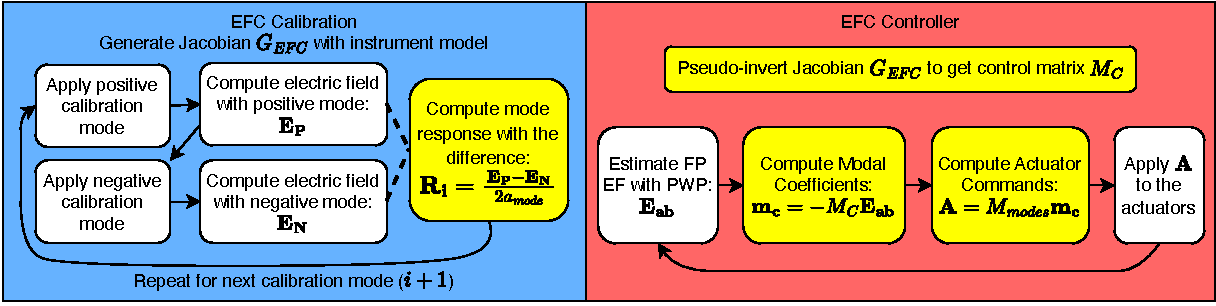
\includegraphics[scale=0.75]{figs-general/efc_flow.pdf}
    \caption{This diagram illustrates the functional steps for model-based EFC. The Jacobian $G_{EFC}$ is constructed by applying positive and negative calibration modes within the model and calculating the electric field at the focal plane. The response/derivative is computed from the difference normalized by the amplitude of the mode applied ($a_{mode}$). The EFC controller uses the pseudo-inverted Jacobian to compute the update to the DM actuators using the estimated electric field $\mathbf{E_{ab}}$. All boxes in yellow indicate a step that is performed computationally.}
    \label{fig:efc-flowchart}
\end{figure}

A critical component to EFC is how the electric field in the focal plane is estimated prior to the actuator command being calculated. While the Self Coherent Camera (SCC) is a method of estimating the focal plane electric field using interference from a reference channel\cite{baudoz2005self}, the common technique proposed for Roman is Pairwise Probing (PWP)\cite{krists-bible}. This method uses at least two linearly independent DM probes to generate phase diversity within the focal plane. Given a model or model-based Jacobian, the difference images of the pairwise probes can be used to estimate the electric field in each pixel of the desired dark hole by solving the equation 
\begin{equation}
\label{eq:pwp}  
\mathbf{\delta_I} = M_{probes} \mathbf{E_{ab}} 
\end{equation} 
\noindent for $\mathbf{E_{ab}}$\cite{give'on-pwp}. Here, $\mathbf{\delta_I}$ is the vector of difference images recorded for each probe and $M_{probes}$ is a matrix with the real and imaginary components of the focal plane electric field contributed by the DM probes. Various implementations of PWP have been developed, including extensions to broadband estimation\cite{redmond-pwp} and implementations of a Kalman filter for improved estimation\cite{groff-pwp-kf}, but all rely on the difference images from pairwise probes. The significant observation leading to iEFC is that the difference images are a linear proxy to the electric field.

\subsection{iEFC}
\label{sec:iefc}
Unlike EFC, iEFC includes no explicit calculation of the electric field within individual iterations of the controller. As described in Haffert et al\cite{haffert-iefc}, iEFC constructs a Jacobian empirically by recording the response for each DM mode in a given set of modes. Figure \ref{fig:iefc-flowchart} demonstrates that each individual response within the Jacobian $G_{IEFC}$ is a double difference where $\mathbf{\delta}$ is the concatenated vector of difference images for the chosen probes. As shown with PWP, the difference images of probes are a linear proxy to the electric field, so minimizing the difference images also minimizes the electric field\cite{haffert-iefc}. The cost function remains very similar except for the fact that instead of $\mathbf{E_{ab}}$, $\mathbf{\delta}$ is minimized with the iEFC Jacobian. 

\begin{equation}
    \label{eq:iefc-1}
    J = |\mathbf{\delta} + G_{IEFC}\mathbf{m_c}|^2  + \lambda|\mathbf{m_c}|^2
\end{equation}

In general, the shape of the final Jacobian should be $N_{probes} N_{pix} \times N_{modes}$ where $N_{probes}$ is the number of probes, $N_{pix}$ is the number of pixels in the control region, and $N_{modes}$ is the total number of modes calibrated. Here, the iEFC controller is extended to utilize two deformable mirrors for application to the Roman Coronagraph by calibrating modes on both DMs while using the first DM for all the probes. Different sets of modes could be utilized for the two DMs, but for simplicity, the simulations here utilize the same modes for each DM. In this case, the number of modes to calibrate increases by a factor of 2. 

\begin{figure}[h]
    \centering
    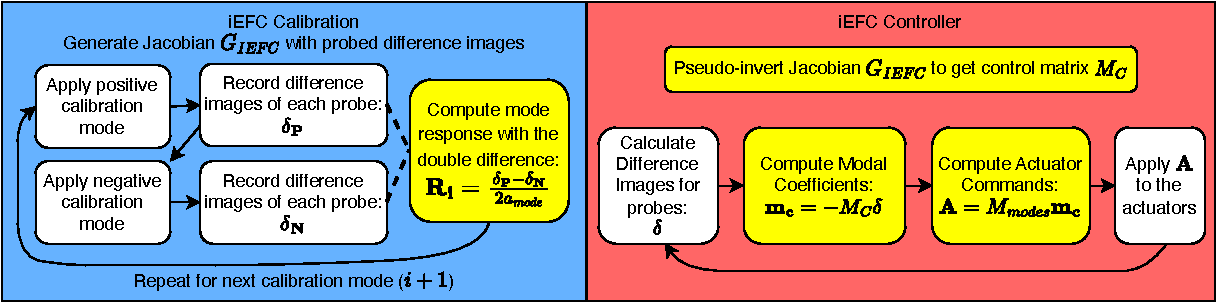
\includegraphics[scale=0.75]{figs-general/iefc_flow.pdf}
    \caption{This diagram illustrates the critical steps for generating a Jacobian for iEFC by calibrating a chosen set of DM modes using difference images of probes concatenated into the vectors $\mathbf{\delta_P}$ and $\mathbf{\delta_N}$. By inverting the Jacobian and measuring $\mathbf{\delta}$ at each iteration, the difference images are minimized to reduce the electric field amplitude. Note that each measurement of $\mathbf{\delta}$ is also normalized by the amplitude of the probe $a_{probe}$.}
    \label{fig:iefc-flowchart}
\end{figure}

With two DMs, $M_{modes}$ is the concatenation of the mode matrix for each DM. This allows for the actuators to be solved for in a single matrix-vector product with the modal coefficients.

\begin{equation}
    \mathbf{A} = M_{modes} \mathbf{m_c} = 
    \begin{bmatrix}
        \mathbf{A_{DM1}} \\
        \mathbf{A_{DM2}}
    \end{bmatrix}
\end{equation}

The two DM iEFC controller is initially tested using an HCIpy\cite{por-hcipy-2018} scalar vortex coronagraph (SVC) model to verify the capability of creating an annular dark hole. The model uses a charge 6 vortex with a 90\% diameter Lyot stop. The wavelength for the simulation is 650nm with two $34\times34$ actuator DMs. The DM pupil is 10mm in diameter with 300mm separation between the DMs (roughly a Fresnel number of 512). The DM modes for which the response is recorded in the Jacobian are Fourier modes with a Fourier sampling of $1\lambda/D$. The probes used are two single actuator pokes of adjacent actuators that are indicated by the white circles on DM1 in Figure \ref{fig:iefc-2dm-annular-dark-hole}. The choice of Fourier modes, sampling, and probes will be expanded upon in Section \ref{sec:mono-iefc}. For now, these modes are significant as they are chosen based on the desired control region such that the total number of modes calibrated is 640. This corresponds to 320 Fourier modes for each DM. This is significantly lower than the total number of actuators, 1904, because the control region does not extend to the maximum controllable spatial frequency of $17\lambda/D$.  The DM solutions and resulting dark hole are presented in Figure \ref{fig:iefc-2dm-annular-dark-hole}. While this result is for an ideal monochromatic vortex coronagraph, the application of iEFC with 2 DMs is found to be suitable for annular dark holes.

\begin{figure}[h]
    \centering
    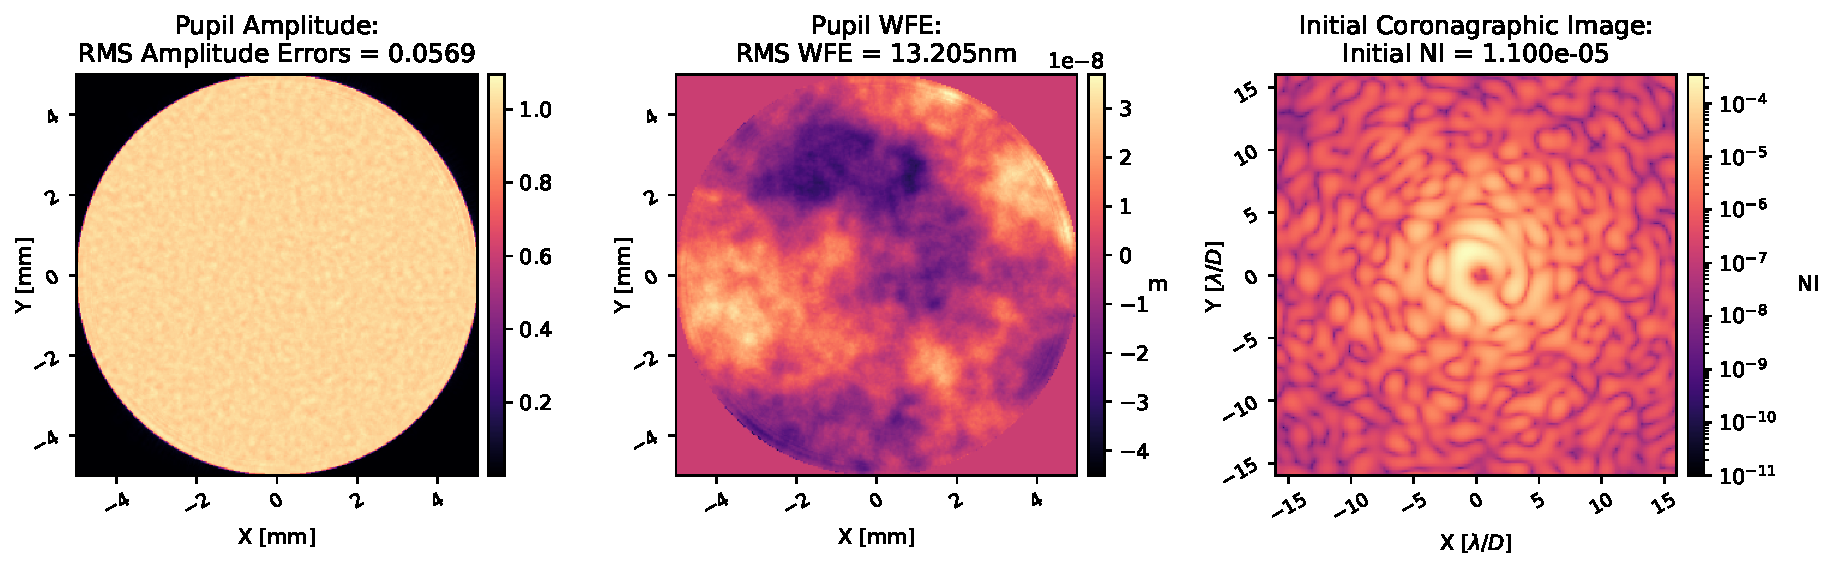
\includegraphics[scale=0.45]{figs-general/hcipy_svc_initial_state.pdf}
    \includegraphics[scale=0.45]{figs-general/hcipy_svc_dark_hole.pdf}
    \caption{Annular dark hole created using iEFC with a scalar vortex coronagraph model. The specified ROI for the dark hole extends from an IWA of 2$\lambda/D$ to $10\lambda/D$. The final mean contrast is measured to be $2.45\times10^{-9}$ after 50 iterations. The two white circles on the first DM indicate the actuators that are used as probes.}
    \label{fig:iefc-2dm-annular-dark-hole}
\end{figure}


\section{Roman SPC Physical Optics Model}
\label{sec:roman-pom}
The optical models used to simulate iEFC for Roman are end-to-end diffraction models that propagate a single wavefront through the entire optical train. This model was created using POPPY\cite{perrin-poppy-2017}; however, it uses the same prescription and data contained within the roman\_phasec\_proper (v1.4) package\footnote{\href{https://sourceforge.net/projects/cgisim/}{https://sourceforge.net/projects/cgisim/}}. The motivation for choosing POPPY was to leverage end-to-end simulations entirely on a GPU as CuPy\cite{cupy_learningsys2017} was recently added as a computation feature in POPPY, greatly reducing simulation times. Both POPPY and PROPER\cite{krist-proper} use a combination of Fresnel and angular spectrum propagation to propagate from optic to optic. The POPPY algorithms have previously been validated by comparisons with results from PROPER\cite{} and the SPC-WFOV model is compared directly to the PROPER model in Figure \ref{fig:spc-wfov-comp} to demonstrate the agreement here. 

\begin{figure}[h]
    \centering
    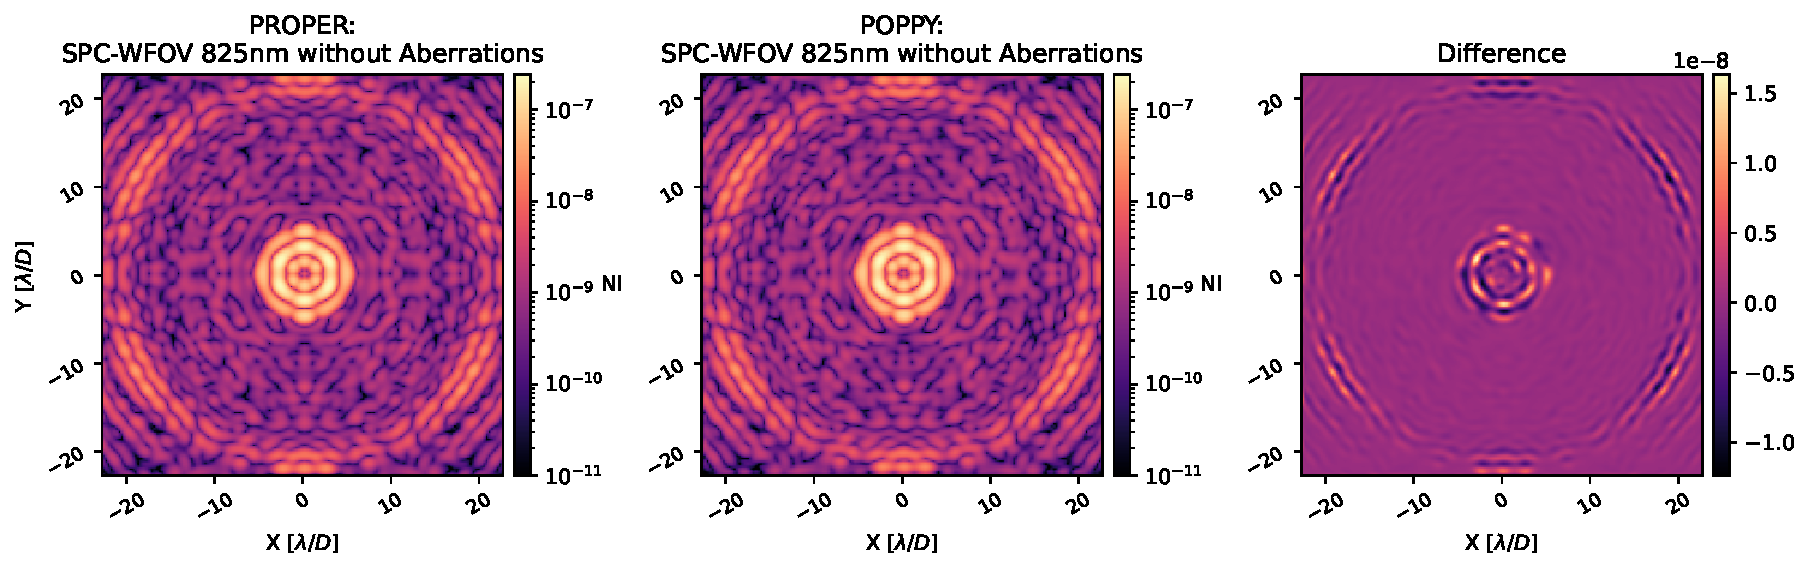
\includegraphics[scale=0.5]{figs-poppy/spc_wfov_825_unaberrated.pdf}
    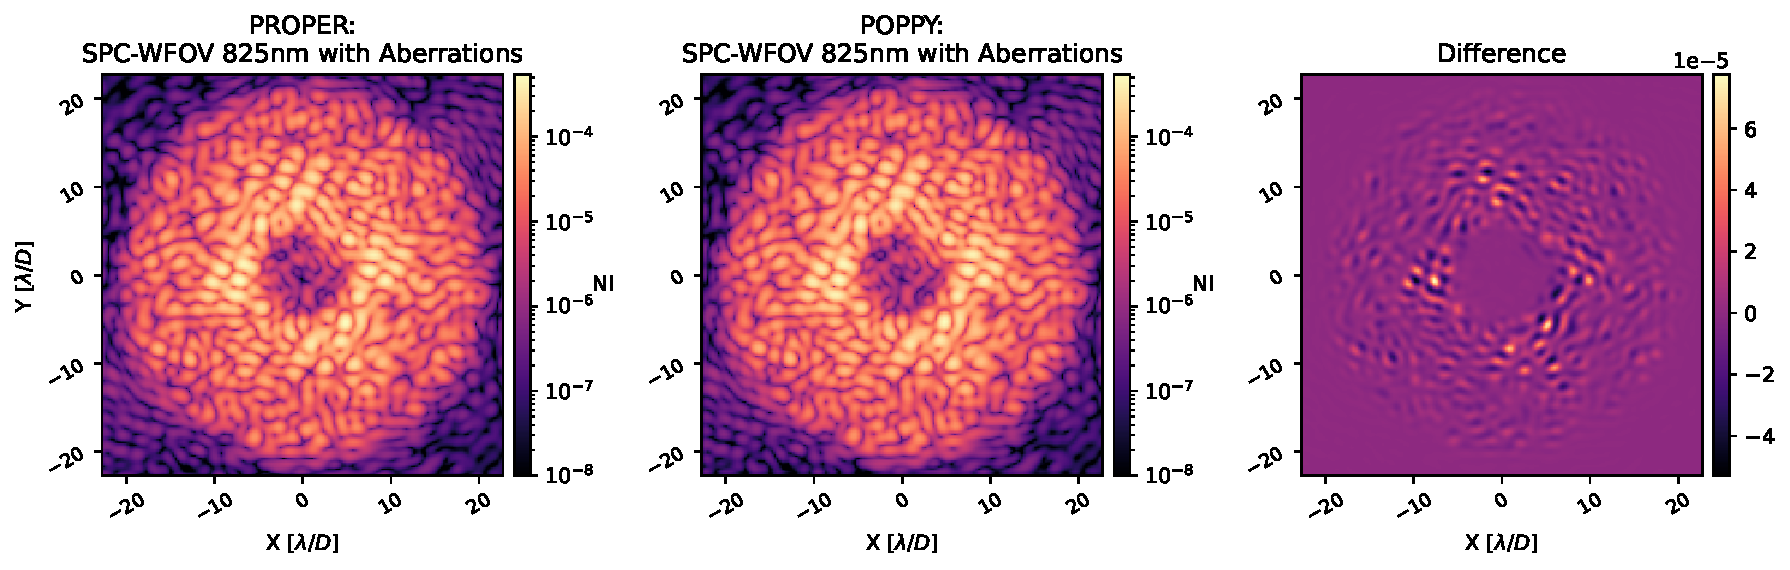
\includegraphics[scale=0.5]{figs-poppy/spc_wfov_825_aberrated.pdf}
    \caption{Comparison of the physical optics model results for the SPC-WFOV mode at 825nm to validate the POPPY model used for simulations. The top row contains no optical aberrations (and no pupil defocus) and illustrates the ideal dark-hole for this coronagraphic mode. The bottom row depicts the same model with aberrations and no DM corrections, resulting in the speckles apparent within the dark-hole region. The mean contrast of the ideal dark-hole is $1.11\times10^{-9}$.}
    \label{fig:spc-wfov-comp}
\end{figure}

The aberrated image of the POPPY model in Figure \ref{fig:spc-wfov-comp} is the initial state that all of the simulations presented begin from. Each DM is completely flat and the initial mean contrast within the desired control region spanning from 5.4$\lambda/D$ to 20.6$\lambda/D$ is $3.04\times10^{-5}$. In this model, there is an additional factor of 2 included in the calculation of optical path difference for the DM surfaces based on the actuator commands given.

For the broadband simulations presented in Section \ref{sec:bb-iefc}, the broadband image is generated by selecting multiple wavelengths within the desired bandpass and propagating a wavefront for each wavelength through the model. This propagation is done in parallel on a GPU using the Ray\cite{moritz2018ray} software for efficient computations. The focal plane wavefronts are incoherently summed to generate the final broadband image. To include estimates of flux, the blackbody equation \begin{equation}\label{eq:blackbody}B_{\lambda} = \frac{2hc^2}{\lambda^5} \frac{1}{\exp{[\frac{hc}{\lambda k_B T}]} - 1}.\end{equation}is used to calculate the spectral radiance for a chosen star in units of W/m$^2$/sr/nm\cite{grant-field-guide-radiometry-2011}. Here, $\zeta$ Puppis is chosen as the reference star because it is a bright star planned to be used for HOWFSC in the Roman Observing Scenarios\cite{krist-spc-wfov-os11}. The spectral radiance of $\zeta$ Puppis is calculated using the temperature of $40,000K$\cite{zeta-pup-temp}. The spectral irradiance is then calculated using the solid angle of the star calculated with the equation \begin{equation} \Omega=2\pi\left(1-\frac{\sqrt{d^2-R^2}}{d}\right)\text{.}\end{equation} Here, $R$ is the radius of the star and $d$ is the distance to the star, both of which are included in Table \ref{tab:zeta-pup-params}. The spectral photon flux is calculated by converting the spectral irradiance using $E=hc/\lambda$. Lastly, the spectral flux is integrated over several sub-bandpasses to estimate the flux for each wavelength that is propagated. 

\begin{table}[h]
    \centering
    \caption{The parameters used to calculate the spectral radiance of $\zeta$ Puppis are presented below along with the final solid angle used to calculate flux.}
    \begin{tabular}{|c|c||} \hline
       Temperature ($T$) & 40,000K\cite{zeta-pup-temp} \\ \hline 
       Radius ($R$) & 14$R_\odot$\cite{zeta-pup-radius} \\ \hline 
       Distance ($d$) & 300parsec\cite{zeta-pup-radius} \\ \hline 
       Solid Angle ($\Omega$) & $1.362\times10^{-17}$sr \\ \hline
    \end{tabular}
    \label{tab:zeta-pup-params}
\end{table}

Figure \ref{fig:blackbody} illustrates an example of the spectrum that is integrated and the broadband images produced for a 10\% bandpass. Here, noise is also included in these images by computing the Poisson distribution for the calculated photons incident on each pixel. Read noise and dark current are also included where the read noise standard deviation is 120\electron/pix and the dark current is 0.05\electron/pix/hour\footnote{\href{https://roman.ipac.caltech.edu/sims/Param_db.html\#coronagraph_mode}{https://roman.ipac.caltech.edu/sims/Param\_db.html\#coronagraph\_mode}}. 

\begin{figure}[h]
    \centering
    \raisebox{-0.5\height}{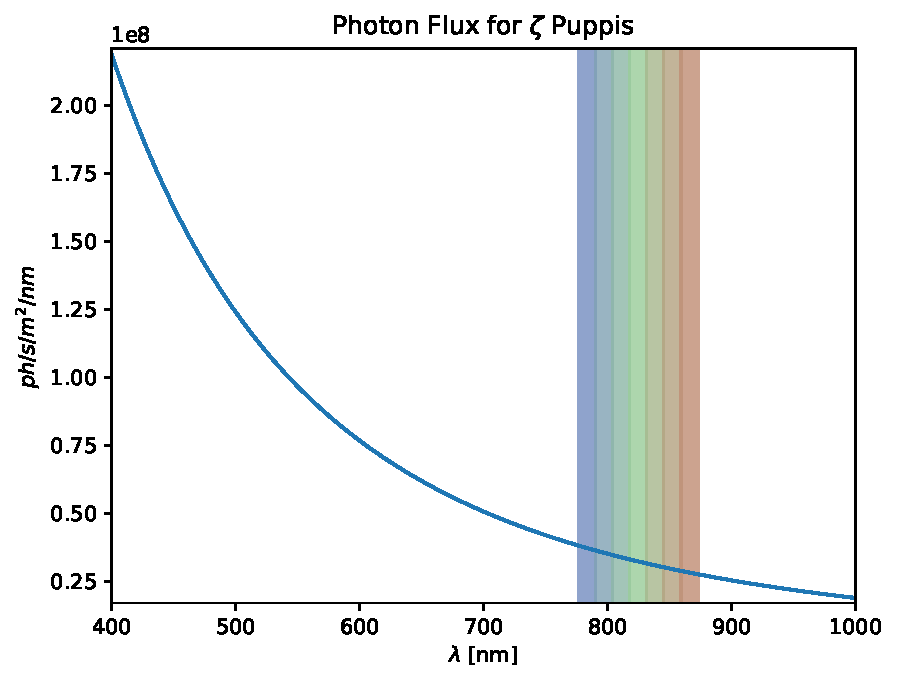
\includegraphics[scale=0.375]{figs-poppy/band4_blackbody_example.pdf}}
    \raisebox{-0.52\height}{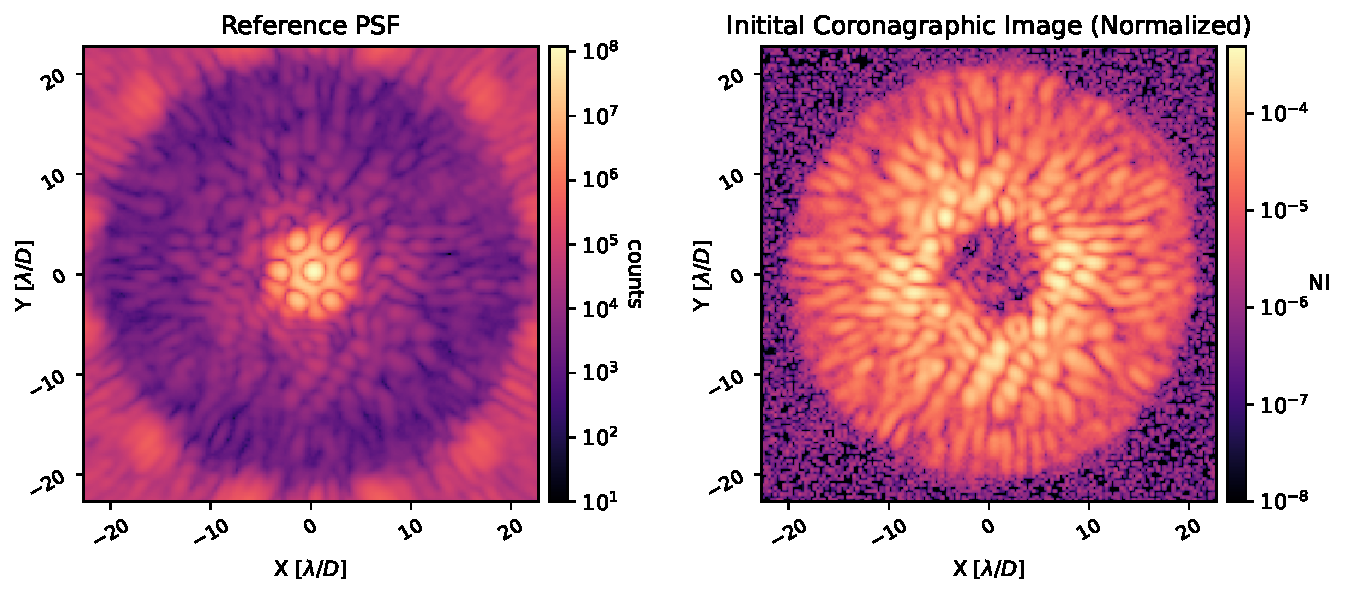
\includegraphics[scale=0.45]{figs-poppy/bb_examples.pdf}}
    \caption{To the left is the spectral flux of $\zeta$ Puppis calculated using the spectral blackbody equation. The highlighted regions illustrate the sub-bandpasses integrated to estimate flux-values for individual wavelengths centered at each sub-bandpass. Note that the peak of the blackbody is located at about 200nm due to the temperature of the star. The middle and right present the simulated broadband images with and without the focal plane mask respectively, but each include the field stop located after the Lyot stop in the optical train. }
    \label{fig:blackbody}
\end{figure}

For this particular frame, the exposure time is 2 seconds. In Section \ref{sec:bb-iefc}, the simulated exposure times are adjusted as necessary while the controller creates a dark hole. Similar to the OS9 simulations for the HLC, the end-to-end physical optics models will include losses from the pupil obstructions and masks, however, losses from the reflectivity or transmission are not included\cite{ygouf-roman-hlc-os9}. Note that no gain is applied to the detector and the quantum efficiency is also not accounted for. Further studies should include a more accurate detector model using stacked frames similar to the methods in OS9 and OS11, but these simulations serve as an initial study to understand if iEFC will be feasible in the presence of high read noise. 


\section{Motivation for iEFC}
\label{sec:motive}
A risk for the Roman Coronagraph will be how well can the model be calibrated to the instrument once the instrument is in orbit. For the SPC-WFOV mode in particular, the transverse position of the Shaped Pupil Mask (SPM) can have a severe impact due to slight misalignments. This is demonstrated by performing EFC simulations with and without a perturbation to the optical model. For these EFC simulations, the end-to-end model is used to compute the EFC Jacobian. Within the EFC controller, PWP is ignored as the optical model is also used to directly calculate the focal plane electric field, effectively simulating a perfect estimation such that these simulations are independent of the estimation technique. The Jacobian is used to perform EFC both with and without a perturbation to the SPM to illustrate the degradation caused by misalignment that was unaccounted for in the model. 

The performance of EFC prior to applying the perturbation to the model is presented in Figure \ref{fig:efc-nominal}. Here, a weighted least-squares regularization of the focal plane pixels is used with the regularization parameter varying between $10^{-1}$ and $10^{-6}$ for 40 iterations. The final solutions yield a mean contrast of $1.58\times10^{-9}$, close to the nominal contrast expected for the unaberrated SPC-WFOV mode presented in Figure \ref{fig:spc-wfov-comp}. Therefore, the EFC algorithm is performing as expected with the optical model unperturbed from the initial state used to compute the Jacobian. 

\begin{figure}[h]
    \centering
    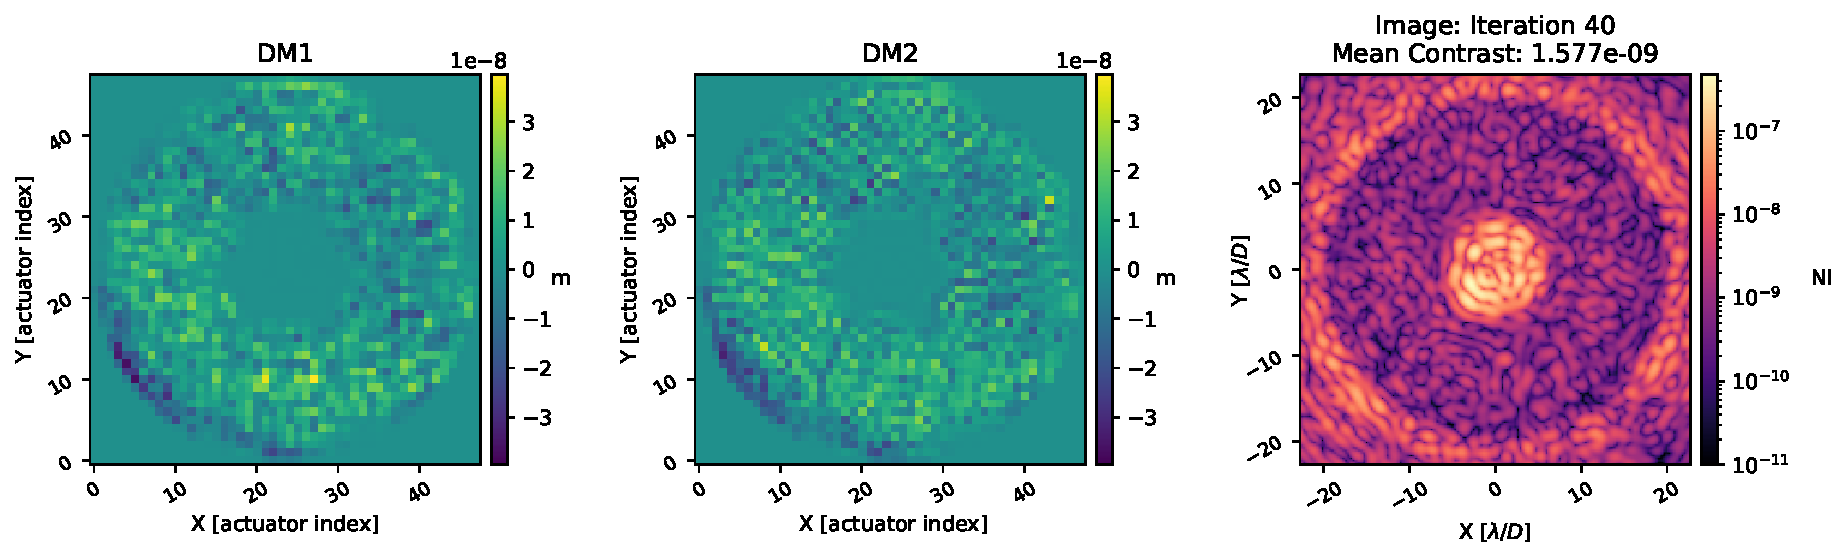
\includegraphics[scale=0.5]{figs-efc/efc_nominal.pdf}
    \caption{Here, the solutions EFC with the coronagraph in the nominal state yield a contrast of }
    \label{fig:efc-nominal}
\end{figure}

The perturbation chosen is a simple shift of the SPM that apodizes the pupil for this mode. Figure \ref{fig:spm-perturbation} illustrates the SPM that is shifted by 5 pixels vertically from the nominal position. In the model, the SPM is sampled with 1000 pixels across the pupil with a sampling of 0.0170mm/pix, making the net shift be 85$\mu\text{m}$. Given that the actuator spacing of the DMs is 0.9906mm and there are 48 actuators across the DM pupil, the active area of the DM is 47.55mm. Therefore, the SPM shift is slightly less than 0.25 actuators. 

\begin{figure}[h]
    \centering
    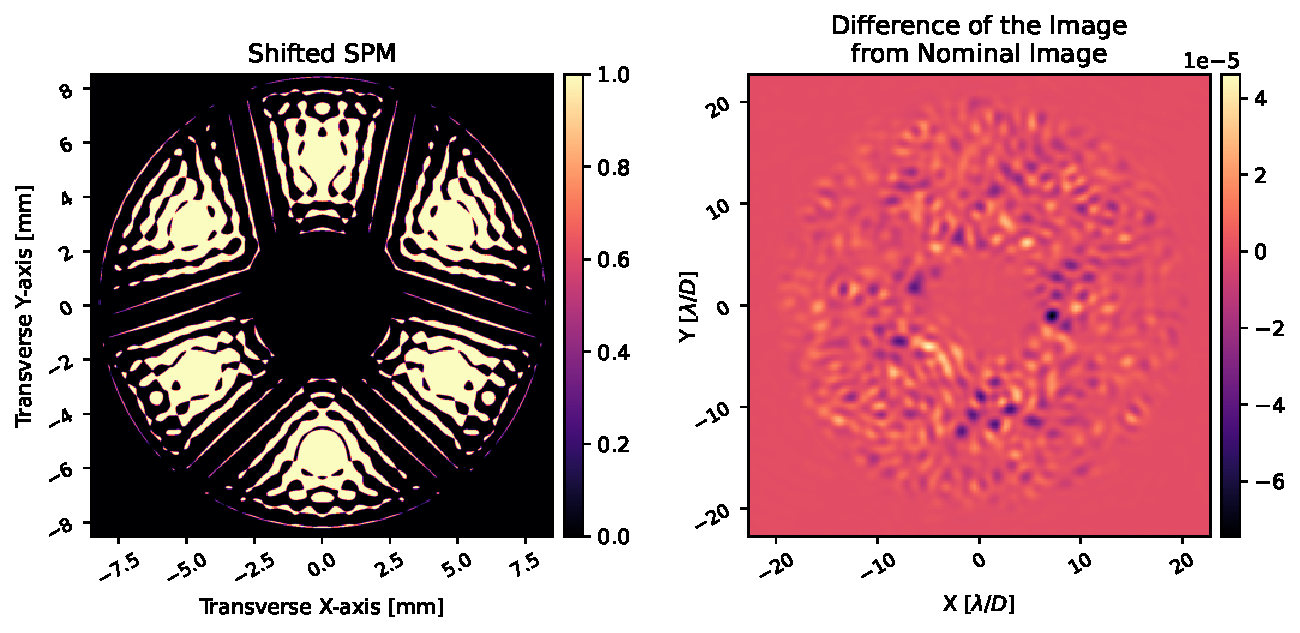
\includegraphics[scale=0.5]{figs-efc/shifted_spm.pdf}
    \caption{The image on the left is the SPM used for the SPC-WFOV mode. Here, the SPM has been shifted by 5 pixels vertically to simulate a misalignment that is not taken into account when generating the Jacobian. The image on the right is the difference in the initial coronagraphic frames with and without this perturbation.}
    \label{fig:spm-perturbation}
\end{figure}

Now, EFC is performed again using this perturbed model acting as the instrument EFC is being performed on. Figure \ref{fig:perturbed-efc} presents the contrast per iteration of EFC as well as the best final result obtained before the algorithm began diverging. The same weighted least-squares regularization was used, however, the regularization parameter was consistently weaker over the iterations. This is because a more strict regularization would cause the solution to diverge earlier in the iterations at which point the resulting contrast would be worse than the best found here. 

\begin{figure}[h]
    \centering
    \raisebox{-0.5\height}{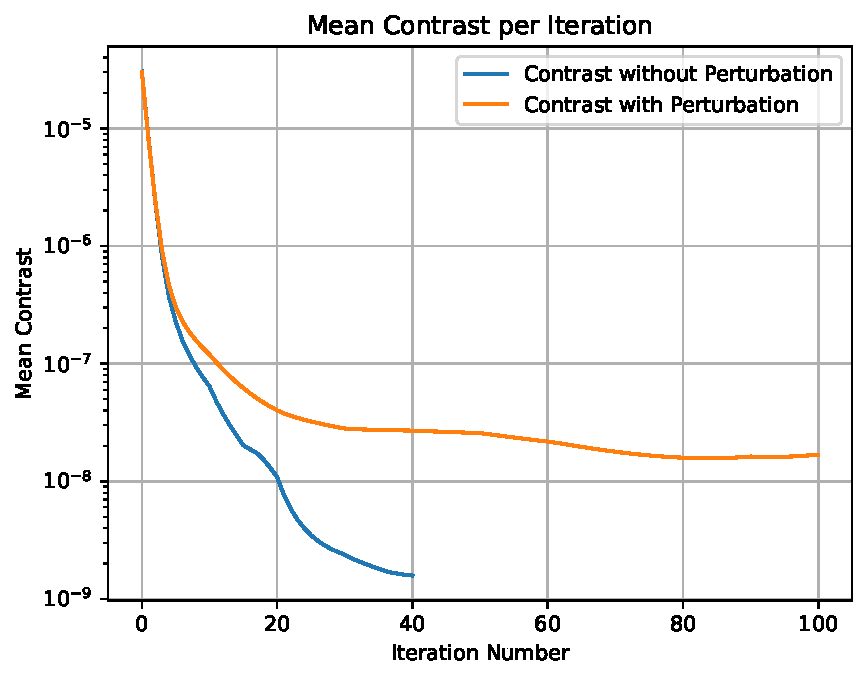
\includegraphics[scale=0.5]{figs-efc/perturbed_contrast.pdf}}
    \raisebox{-0.5\height}{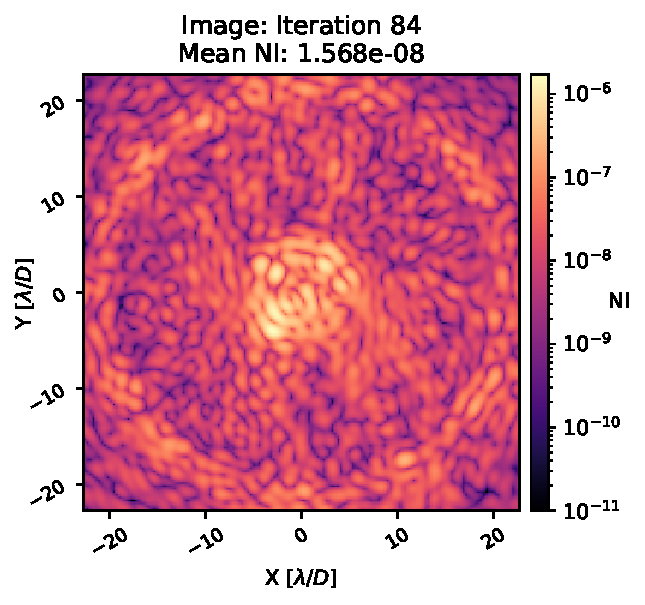
\includegraphics[scale=0.6]{figs-efc/perturbed_best_image.pdf}}
    \caption{The contrast per iteration along with the image from the iteration with the best contrast}
    \label{fig:perturbed-efc}
\end{figure}

Without sophisticated methods of determining the instrument error such that it can be accounted for when calculating a Jacobian with the optical model, EFC can be limited by errors such as this misalignment of the SPM or an accumulation of smaller perturbations within the instrument. An expectation-maximization technique detailed in Sun et al.\cite{sun-system-id-2018} has been one proposed method of recovering the state of a system to improve the model, however, iEFC is another method that can account for a perturbation such as this misalignment as will be demonstrated in the next section. 

\section{Monochromatic iEFC Results}
\label{sec:mono-iefc}
Using the SPC-WFOV mode at 825nm, the iEFC Jacobian is generated for three sets of modes: individual actuator pokes, Fourier modes, and Hadamard modes. In each case, the same probes are used to generate the difference images of each calibration mode. These are analogous to the same probes that could be used for PWP. Figure \ref{fig:example-modes} shows an example of a Hadamard mode and a Fourier mode with the single actuator probes highlighted in red on each image. Each actuator probe is approximately a narrow Gaussian in the pupil plane, so the response of the probe in the focal plane is a broad Gaussian spanning the desired control region. For one-to-one comparisons, the amplitude applied to each calibration mode is 10nm and the amplitude of the probes is 25nm. 

\begin{figure}[h]
    \centering
    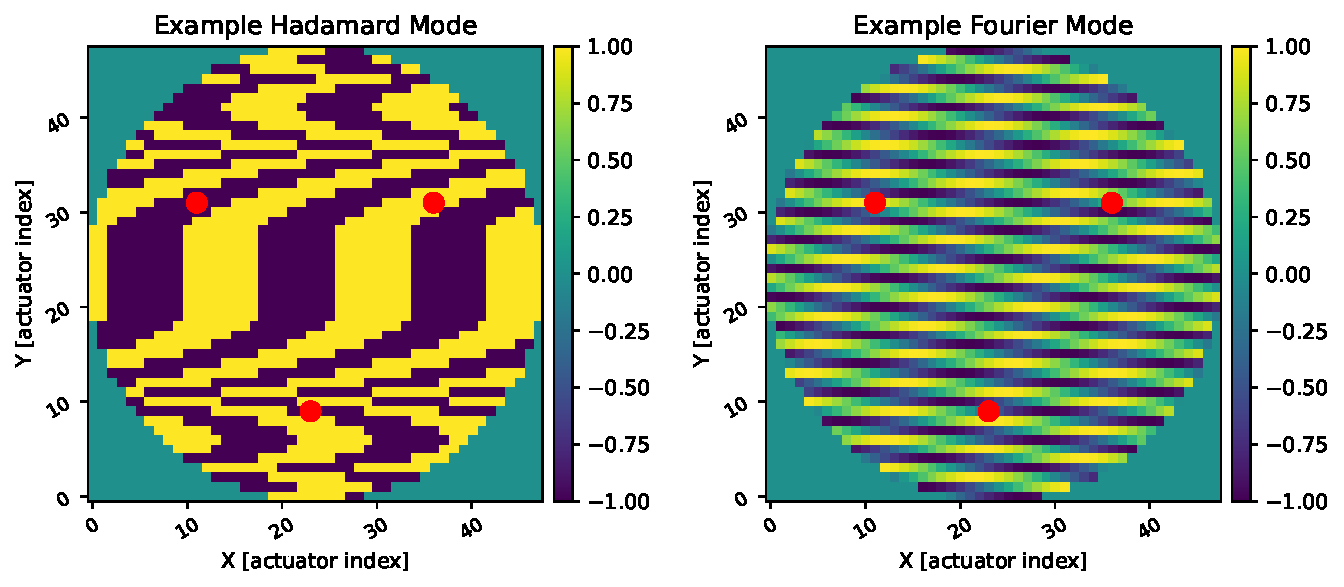
\includegraphics[scale=0.6]{figs-general/example_modes.pdf}
    \caption{The images above depict examples of a Hadamard mode and a Fourier mode. The actuators indicated in red are those used as single actuator probes for which the difference images are measured.}
    \label{fig:example-modes}
\end{figure}

In Potier et al\cite{potier-comparing-fpwfs}, it was demonstrated that using two actuator pokes as probes for estimation of the electric field with PWP is most optimal when the actuators are neighbors. This is because the inverse problem for estimation is well-posed across the field of view, except for a narrow segment across the focal plane that extends normal to the line connecting the two actuators (see Figure 4 in Potier et al.\cite{potier-comparing-fpwfs}). For iEFC, the single actuator probes are similarly important as the difference images act as a linear proxy to the electric field. Given that an annular dark hole is desired here, the region where the inverse problem is ill-posed can lead to poor performance of iEFC. This can be noticed in the simulation with the SVC presented in Figure \ref{fig:iefc-2dm-annular-dark-hole} where there is a narrow region along the y-axis of the focal plane where the iEFC controller has degraded performance.

In addition, because the DM modes desired for wavefront control are applied simultaneously with the probes and the physical response for DM actuators is nonlinear, the slope of the focal plane response that is measured and stored in the Jacobian is greater for those actuators used in the probe commands. This is because the response of a mode is normalized by the amplitude applied during calibration, $a_{mode}$, but the actuators used in the probes use more stroke during the measurement. This is demonstrated by the plot and measured RMS responses found in Figure \ref{fig:poke-dm-response}. During the control loop, those actuators subsequently use more stroke. This will be referred to as print-through of the probes. Using two actuators neighboring each other exacerbates this issue of print-through as a very localized region of the DM will use a large amount of stroke. To avoid both issues of an ill-posed region in the focal plane and the exacerbated print-through affect, three probes were chosen to perform iEFC. The exact choice of probes is presented in Figure \ref{fig:example-modes}.

\begin{figure}[h]
    \centering
    % \raisebox{-0.51\height}{\includegraphics[scale=0.28]{figs-spc-825/dm_mask.png}}
    \raisebox{-0.52\height}{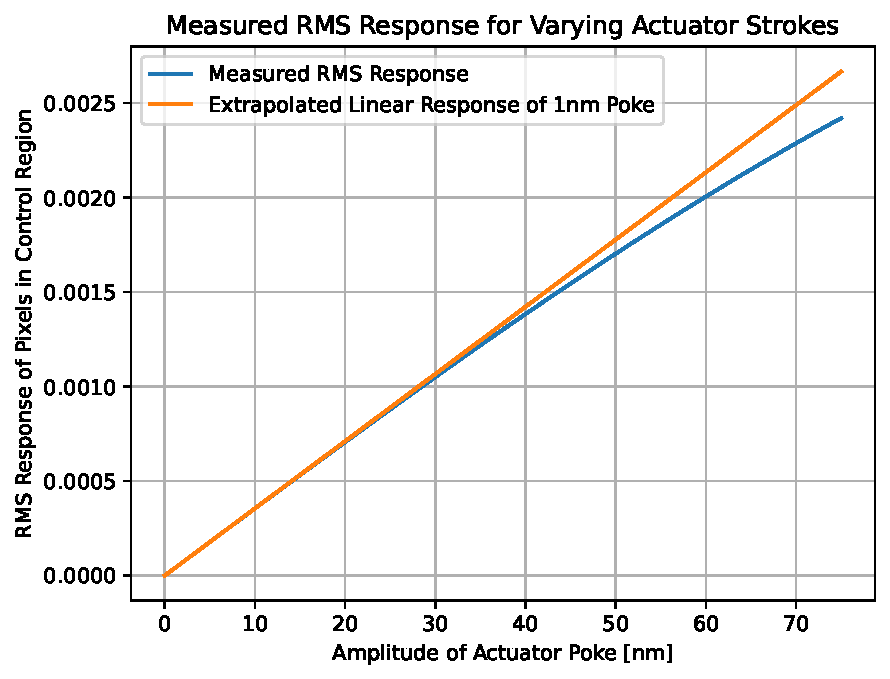
\includegraphics[scale=0.4]{figs-spc-825/nonlinear_response.pdf}}
    \raisebox{-0.5\height}{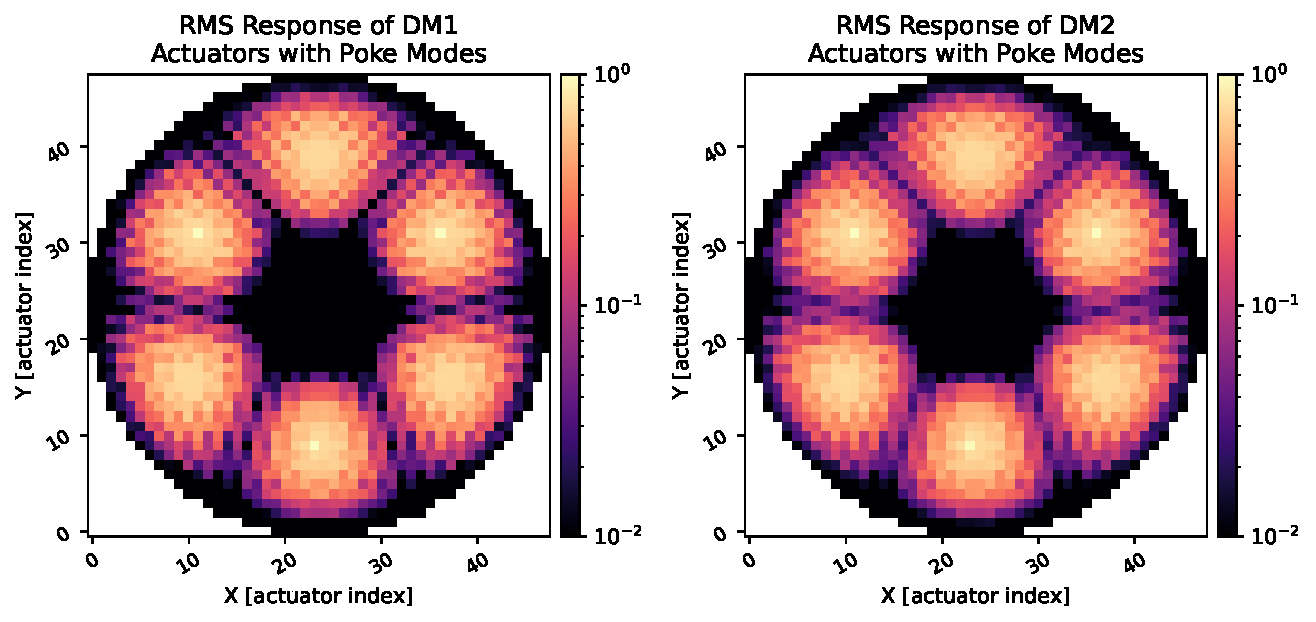
\includegraphics[scale=0.45]{response-maps/poke_mode_responses.pdf}}
    \caption{Here, the plot on the left illustrates the nonlinear response of the electric field to a single actuator poke. The images in the middle and to the right illustrate the RMS response of all calibrated actuators within the control region using single actuators as the modal basis. The RMS responses are normalized to the maximum actuator response.}
    \label{fig:poke-dm-response}
\end{figure}

Using single actuator modes for iEFC, a total of 3608 single actuators are calibrated with 1804 actuators per DM. In theory, the actuators known to have a relatively minimal response due to the obscuration by the SPM can be truncated from the calibration modes prior to calibration, but those actuators are included in these simulations for completeness.

After 85 iterations with the single Jacobian, a mean contrast of $2.55\times10^{-9}$ was attained with the iEFC controller. The DM solutions and subsequent dark-hole are presented in Figure \ref{fig:spc-825-poke_modes}. Throughout the iterations, the regularization parameter was varied every 3 to 5 iterations to avoid local minima of the weighted-least-squares cost function. This is repeated for the results with Fourier and Hadamard modes further below. Here, the print-through of the probes is apparent on each DM due to the proximity of the second DM to the pupil-plane. This is noticed in the results with Fourier and Hadamard modes as well.

\begin{figure}[h]
    \centering
    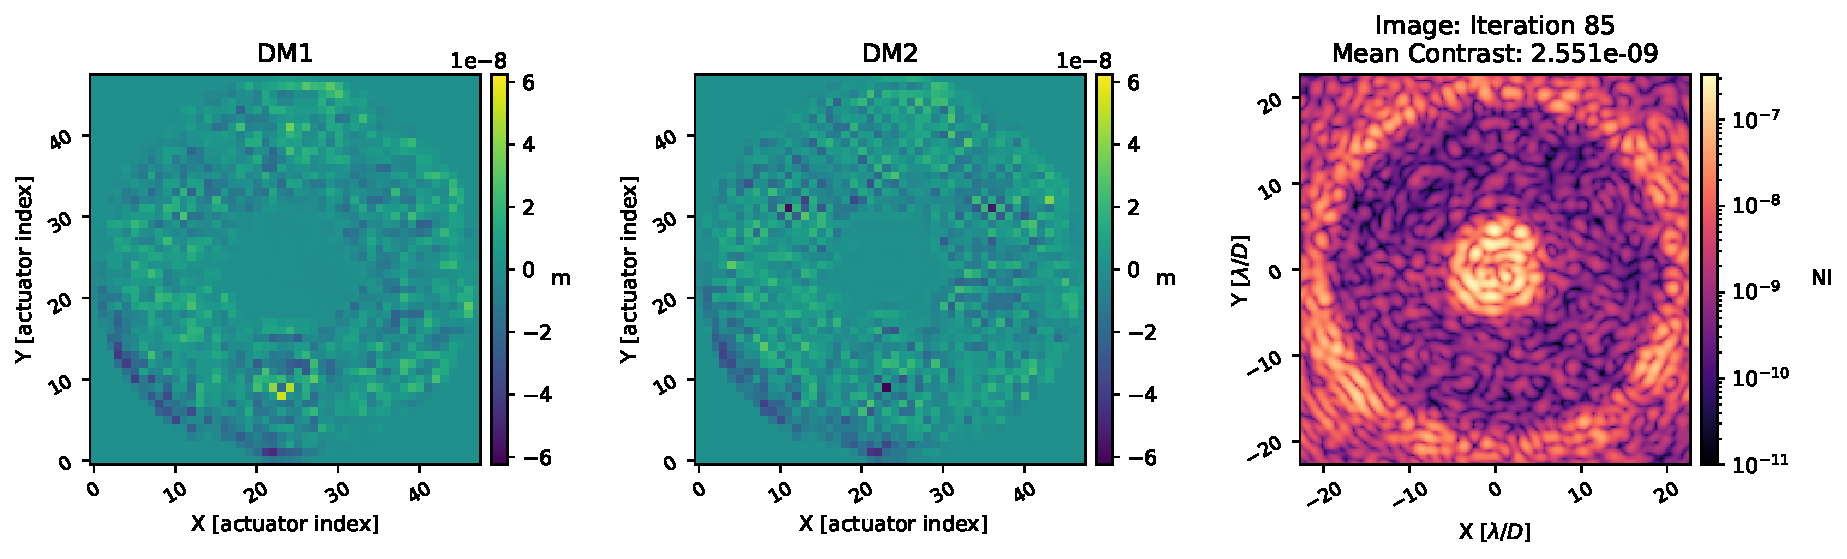
\includegraphics[scale=0.5]{figs-spc-825/spc_825_poke_modes_poke_probes.pdf}
    \caption{The solution of iEFC using individual actuators as the DM modal basis attained a dark hole with a mean contrast of $2.55\times10^{-9}$.}
    \label{fig:spc-825-poke_modes}
\end{figure}

When calibrating Fourier modes, the response of 3512 modes is measured. This number of modes iss determined by the size of the desired control region, which spans from 5.4$\lambda/D$ to 20.6$\lambda/D$, and the Fourier sampling of the modes that was 0.85$\lambda/D$. Here Fourier sampling refers to the angular separation of the spatial frequency between separate modes. Each DM uses 1756 modes of which half are cosines while the other half are sines such that the modal basis spans the desired range of actuator modes. For Hadamard modes, a total of 4096 modes are chosen based on the number of actuators within the DM pupil. With 1804 actuators per DM, a set of 2048 Hadamard modes is initialized. This is because Hadamard modes are generated in powers of 2, so the next highest power of 2 is chosen to ensure a basis that spans the range of DM actuators. Figure \ref{fig:had-fourier-responses} presents the RMS response of each actuator for both Fourier and Hadamard modes. The RMS response of each actuator is again computed using the matrix of calibration modes to decompose each mode's response into the response of individual actuators. 

\begin{figure}[h]
    \centering
    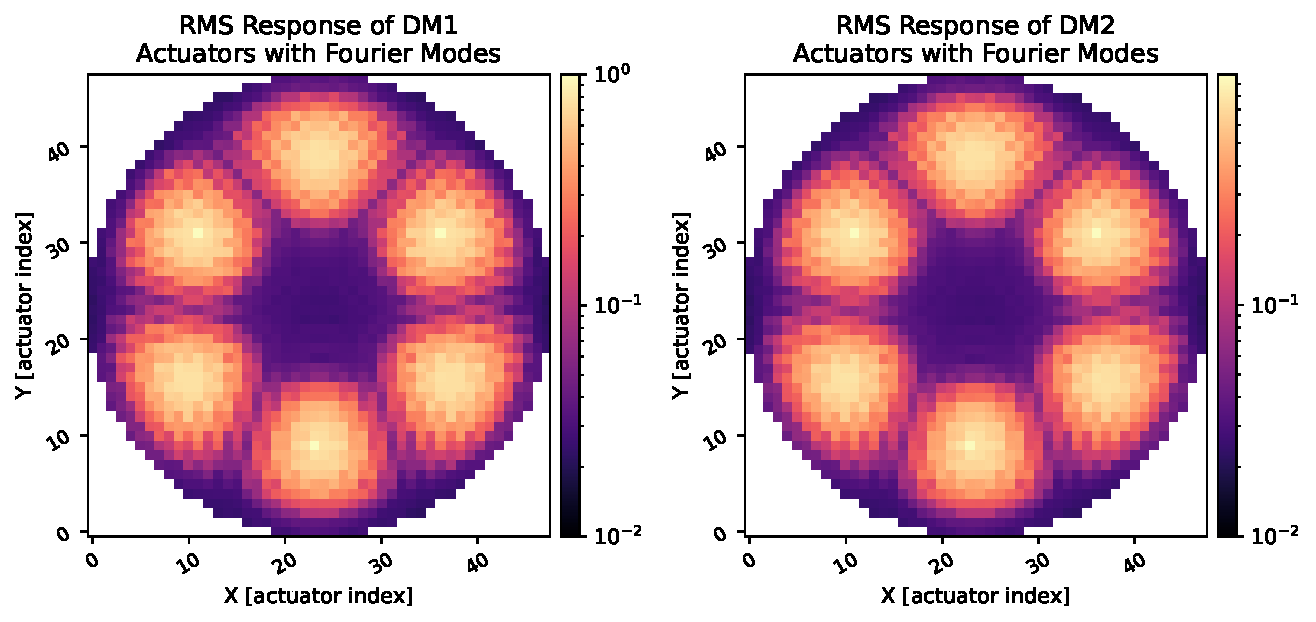
\includegraphics[scale=0.35]{response-maps/fourier_mode_responses.pdf}
    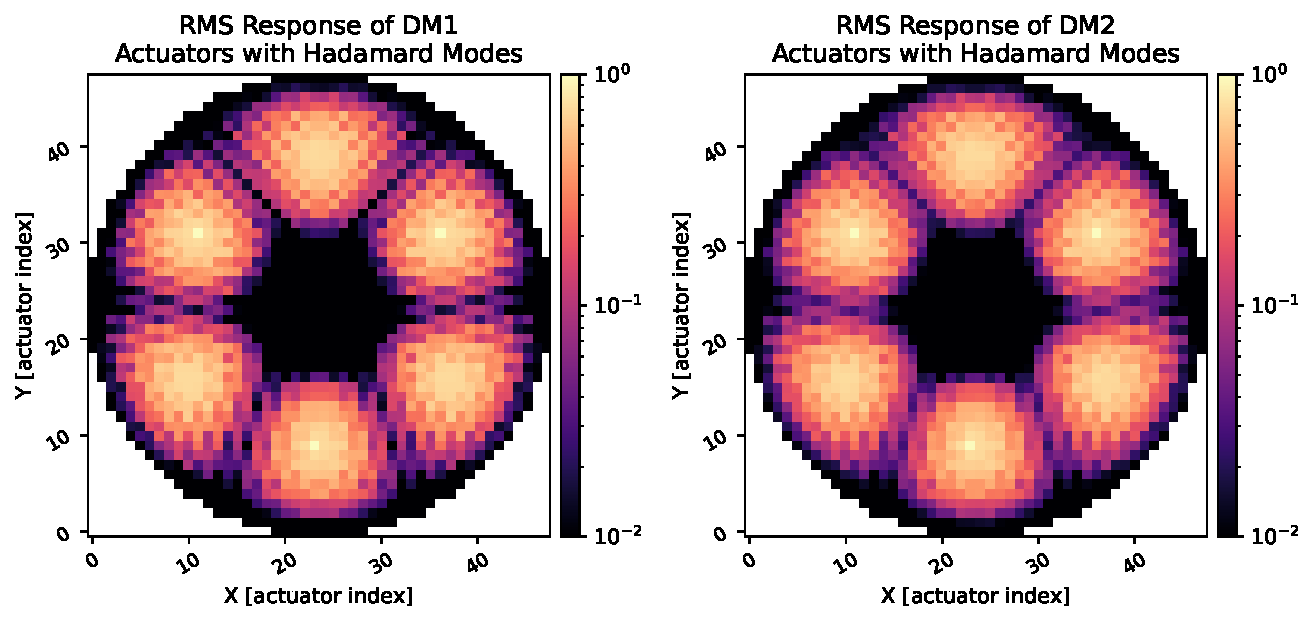
\includegraphics[scale=0.35]{response-maps/had_mode_responses.pdf}
    \caption{Here, the normalized RMS response of each actuator within the control region using Fourier (left) and  Hadamard (right) modes is presented. The response of each mode is decomposed into the individual actuator responses using the matrix of calibration modes $M_{modes}$. Each response is normalized to the actuator with the maximum response (for the respective modes). For the Fourier modes, the maximum response was about $1400\times$ greater than the maximum response using single actuator modes and the maximum response using Hadamard modes was about $2000\times$ greater. This is expected given that Fourier and Hadamard modes concentrate the response within the desired control region more effectively and more Hadamard modes are used than Fourier modes.}
    \label{fig:had-fourier-responses}
\end{figure}

The final iEFC solutions obtained with the Fourier modes are presented in Figure \ref{fig:spc-825-fourier_modes}. Here, the final iteration is 41 because the controller began diverging afterwards. The minimum reached was $2.96\times10^{-8}$, indicating the Fourier modes are a significantly worse choice than single actuator modes. Additional simulations were performed using a reduced calibration amplitude of 2.5nm as well as a simulation with a Fourier sampling of $0.8\lambda/D$. The denser Fourier sampling results in a total of 3992 Fourier modes being calibrated. Both these simulations yielded similar results with no noticeable improvements in final contrast or convergence. 

\begin{figure}[h]
    \centering
    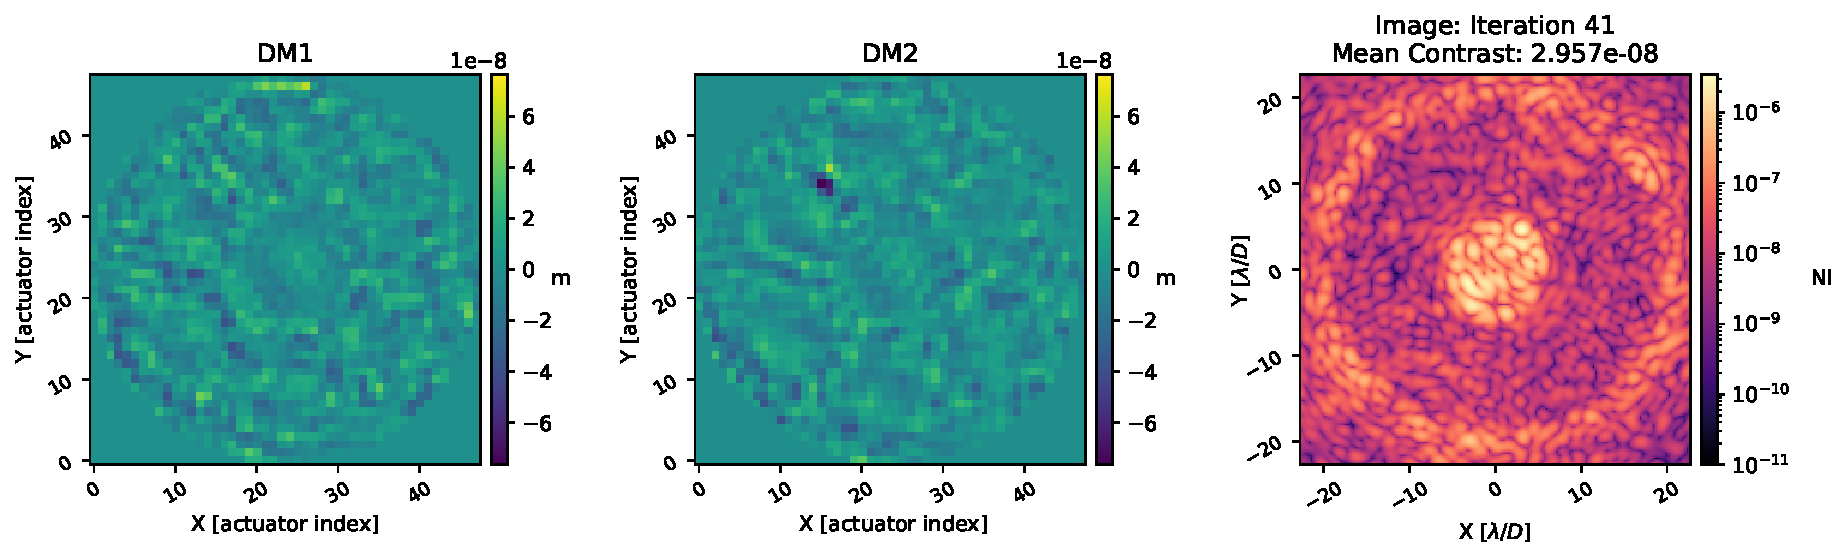
\includegraphics[scale=0.5]{figs-spc-825/spc_825_fourier_modes_poke_probes.pdf}
    \caption{The best contrast achieved with the Fourier modes was $2.96\times10^{-8}$ after 41 iterations. Further iterations began diverging from a minimal solution, indicating that Fourier modes are not an effective choice for the SPC-WFOV mode.}
    \label{fig:spc-825-fourier_modes}
\end{figure}

While the Fourier modes have poor performance for the SPC-WFOV mode when compared to the effectiveness for the SVC model from Section \ref{sec:iefc}, the Hadamard modes have much better performance. Shown in Figure \ref{fig:spc-825-had_modes}, the solutions of the final monochromatic simulation with Hadamard modes yielded the best average contrast of $2.14\times10^{-9}$. Significantly, the Hadamard modes also converged to a better contrast within about half the iterations required with the single actuator modes. Figure \ref{fig:convergence} illustrates this by plotting the mean contrast per iteration using each set of modes. 

\begin{figure}[h]
    \centering
    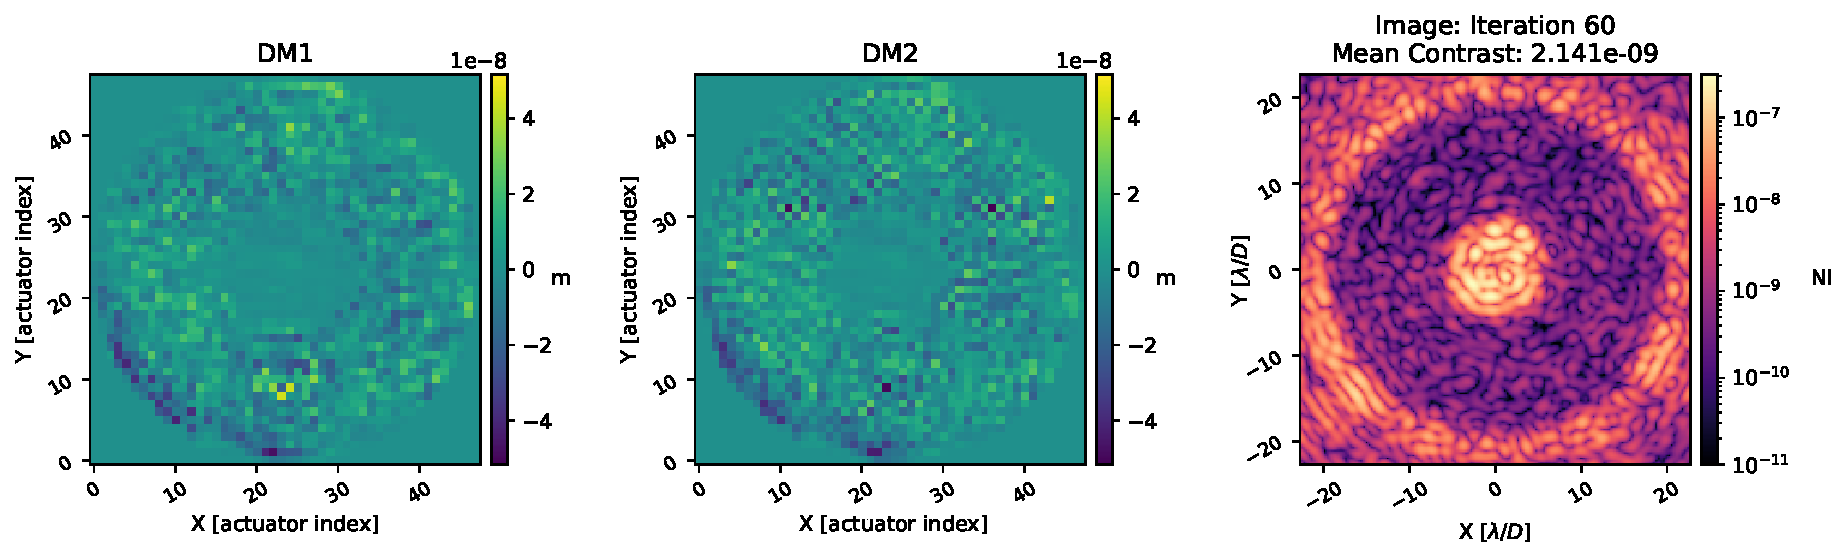
\includegraphics[scale=0.5]{figs-spc-825/spc_825_had_modes_poke_probes.pdf}
    \caption{The two DM solutions of iEFC with Hadamard modes yielded a mean contrast of $2.14\times10^{-9}$ after 60 iterations. The more rapid convergence of Hadamard modes when compared to the single actuator modes makes them the preferred choice for this coronagraph mode.}
    \label{fig:spc-825-had_modes}
\end{figure}

\begin{figure}[h]
    \centering
    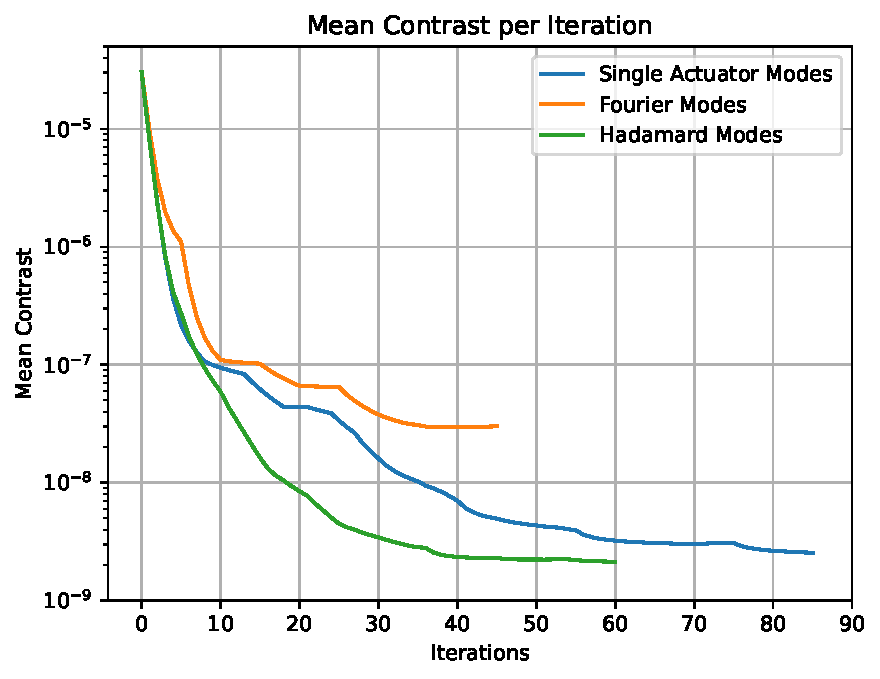
\includegraphics[scale=0.8]{figs-spc-825/contrast_per_iteration.pdf}
    \caption{The contrast attained using each of the three sets of modes demonstrating that Hadamard modes were the optimal choice for the SPC-WFOV.}
    \label{fig:convergence}
\end{figure}

Now, iEFC was performed with the same SPM perturbation discussed in Section \ref{sec:motive}. Given that the iEFC Jacobian is generated empirically, the perturbation was included when computing the Jacobian using the same Hadamard modes and single actuator probes. The final solution of iEFC achieved a contrast of $4.15\times10^{-9}$. While this contrast is worse than that obtained with the unperturbed model, it is better than the contrast of $1.57\times10^{-8}$ achieved with the perturbation included during EFC. Significantly, iEFC achieved this in 50 iterations while EFC required 84 to achieve the best contrast before diverging. 

\begin{figure}[h]
    \centering
    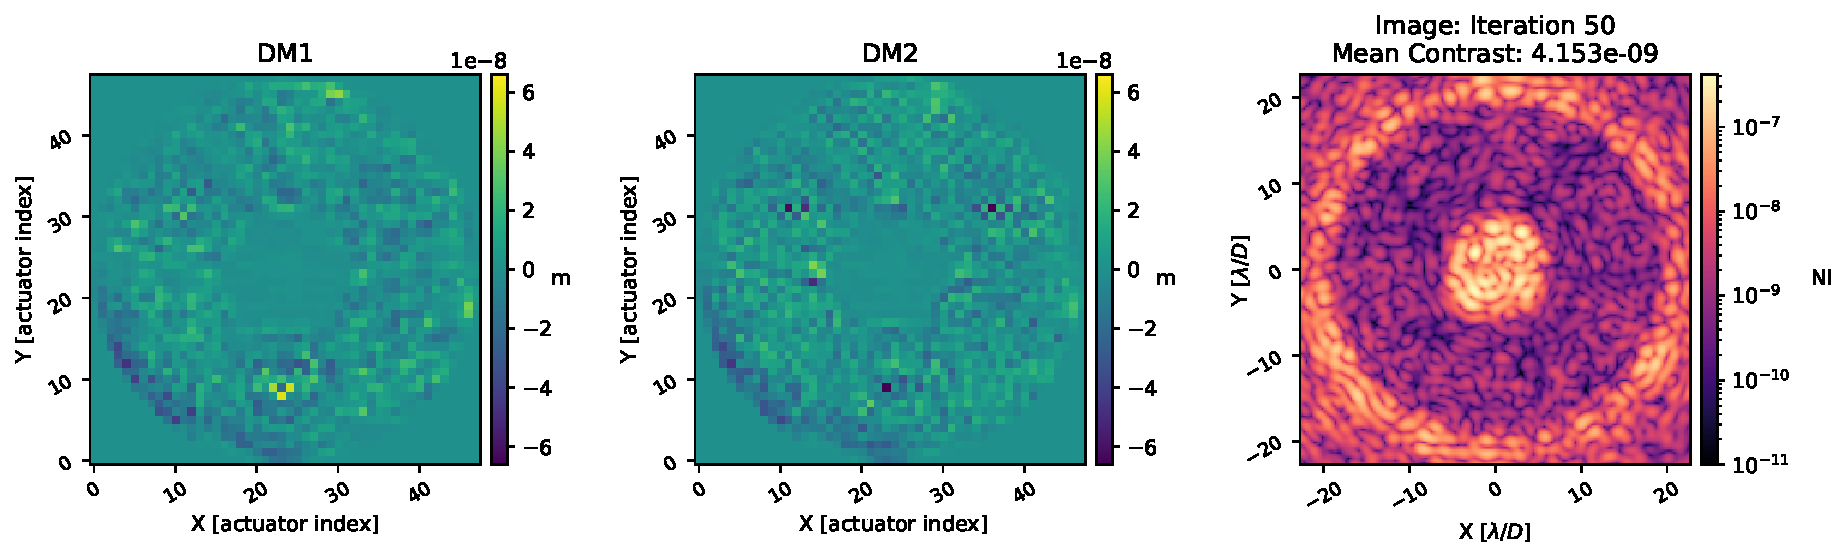
\includegraphics[scale=0.5]{figs-spc-825/iefc_perturbed_best_image.pdf}
    \caption{Above are the iEFC solutions with the misaligned SPM. While the contrast attained in the presence of the perturbation is worse than without, the performance when compared to EFC is significantly improved.}
    \label{fig:iefc-perturbed}
\end{figure}

\section{Broadband iEFC Simulations with Noise}
\label{sec:bb-iefc}
Informed by the monochromatic simulation results, broadband simulations with the single actuator and Fourier modes are not included. The chosen bandpass to simulate is the 3.6\% (FWHM) band 4b filter centered at 825nm\cite{krists-bible}. This choice is made due to the difficulty in performing wavefront control over a large bandpass given the blurring of speckles that occurs at larger angular separations. To effectively perform wavefront control over a wider bandpass, multiple narrow bandpasses can be calibrated and concatenated into a single Jacobian\cite{haffert-iefc}, but the demonstration here is for a simple narrow band filter. Each simulated image is an incoherent sum of three wavefronts with wavelengths spanning the chosen bandpass. These three wavelengths are 813nm, 825nm, and 837nm, for which the flux of each is estimated assuming the reference to be $\zeta$ Puppis given it has been used as a case study for the observing scenarios. Here, no gain is being applied to the detector and the amplitude of the calibration modes and probes remain the same as in the monochromatic simulations. Figure \ref{fig:noisy-responses} illustrates why the noisy images can degrade the accuracy of the Jacobian as the obscured actuators now have a larger and relatively constant response caused by the noise sources.

\begin{figure}[h]
    \centering
    \raisebox{-0.5\height}{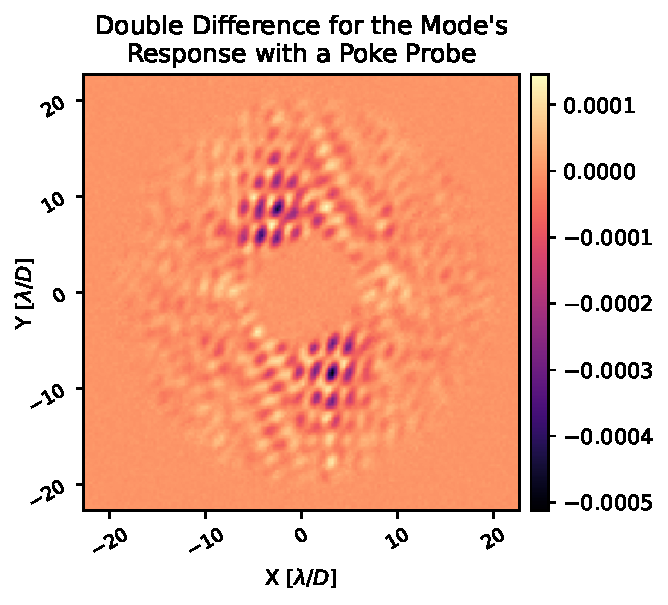
\includegraphics[scale=0.5]{figs-spc-band4b/dd_for_poke_probe.pdf}}
    \raisebox{-0.48\height}{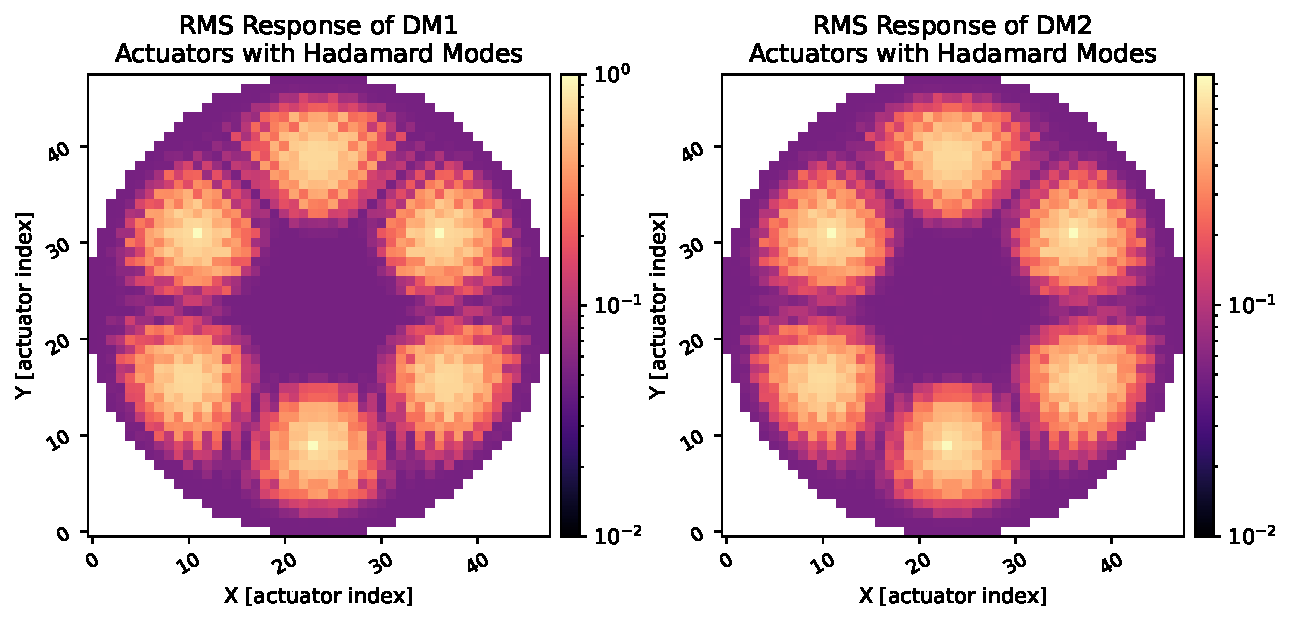
\includegraphics[scale=0.45]{figs-spc-band4b/had_modes_3pokes_responses.pdf}}
    \caption{To the left is an example of a double difference image for the same example Hadamard mode from Figure \ref{fig:example-modes}. The noise in the image demonstrates why the Jacobian accuracy is degraded as the noise is now included when computing the response. In the middle and right are the RMS responses of each actuator using the Hadamard modes to further illustrate how noise increases the response of the obstructed actuators.}
    \label{fig:noisy-responses}
\end{figure}

For the first simulation using the same three actuator pokes as probes, the exposure time chosen for individual frames during calibration is 2s. Using this exposure time, the mean number of incident photons per pixel is 665. With the photon noise, a read noise of 120\electron/pix and a dark current of 0.05\electron/pix/hour, the SNR for the initial image without a probe or calibration mode applied is 23.7. With this exposure time, the estimated calibration time is 27.3 hours for 12 images per Hadamard mode calibrated. This estimated calibration time is similar to the total observation time of 25hrs for the science target from OS11 simulations of the SPC-WFOV mode\cite{krist-spc-wfov-os11}. During the control-loop, exposure times are increased as contrast is gained. Here, the final exposure time after 50 iterations is 20min. With three probes, six images are required per iteration, so the total estimated time for each iteration is 2 hours. The solutions exhibited in Figure \ref{fig:spc-band4b-poke-probes} yield a final contrast of $4.44\times10^{-8}$. 

\begin{figure}[h]
    \centering
    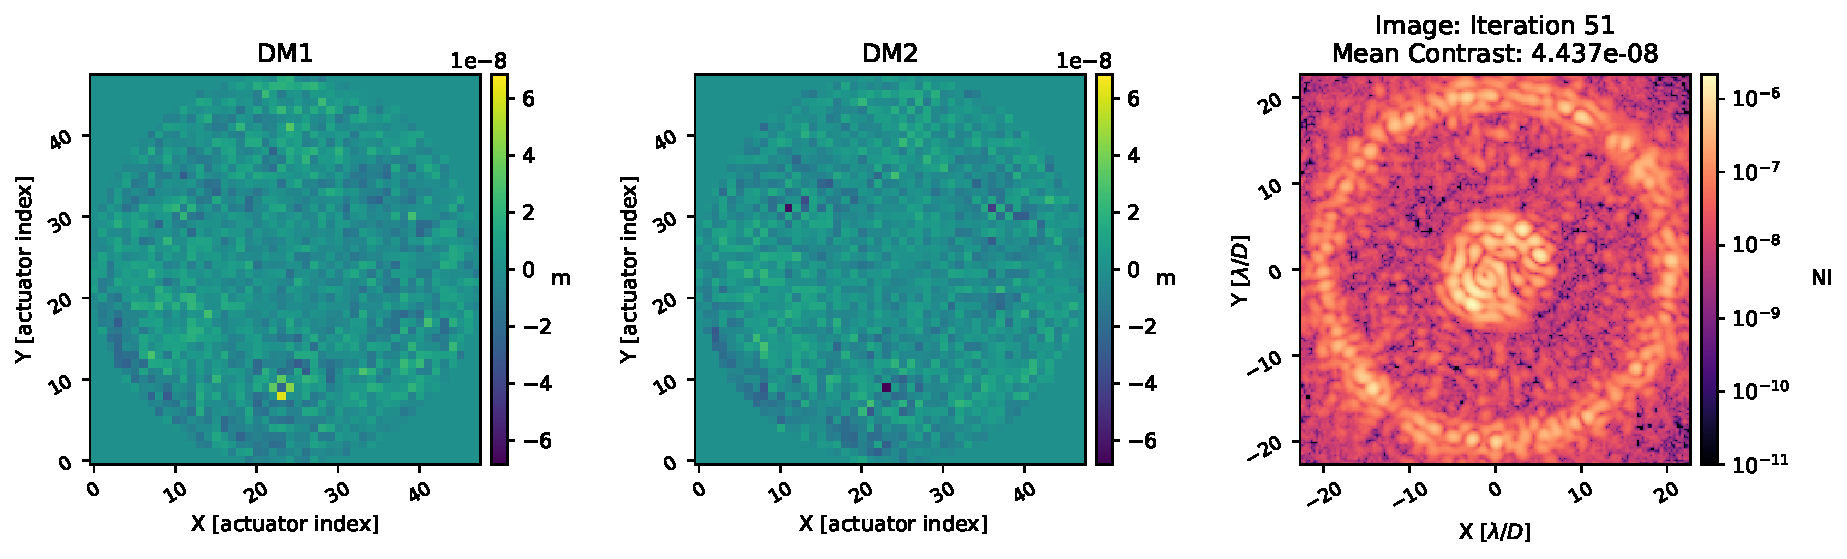
\includegraphics[scale=0.5]{figs-spc-band4b/had_modes_3pokes.pdf}
    \caption{Using the three actuator probes, the DM solutions yield a final contrast of $4.44\times10^{-8}$. Notably, the noise of the measured responses results in increased stroke of the obstructed actuators. Further iterations yielded minimal improvement as the controller is limited by the noise in the Jacobian.}
    \label{fig:spc-band4b-poke-probes}
\end{figure}

The relatively poor performance of this simulation is attributed to the low SNR attained with the chosen single actuator probes. A possible remedy for this could be to use longer exposure times during calibration, but with the calibration requiring 27hours already, this is not the desired solution. Another solution could be to use larger amplitude pokes, but this will exacerbate the issue of print through due to the nonlinear response of large DM strokes. The chosen solution is to use a set of Fourier probes instead of the single actuator probes. Illustrated in Figure \ref{fig:spc-band4b-fourier-probe-examples}, each Fourier probe is a weighted sum of the cosine and sine modes from the complete set of Fourier modes spanning the control region. The probes are then shifted to an unobstructed area of the DM similar to the single actuator pokes to maximize the focal plane response. The same amplitudes of 25nm for the probes and 10nm for the Hadamard modes were used to generate the Jacobian. The example of a double difference image in Figure \ref{fig:spc-band4b-fourier-probe-examples} demonstrates that the Fourier probe generates a higher amplitude response than the single actuator probes in order to mitigate the affects of noise. For this particular Hadamard mode, the peak to valley of the double difference measurement in units of normalized intensity is $6.58\times10^{-4}$ with the single actuator probe. With the Fourier probe, the peak to valley is $1.69\times10^{-3}$, roughly $2.5\times$ greater. 

\begin{figure}[h]
    \centering
    \raisebox{-0.5\height}{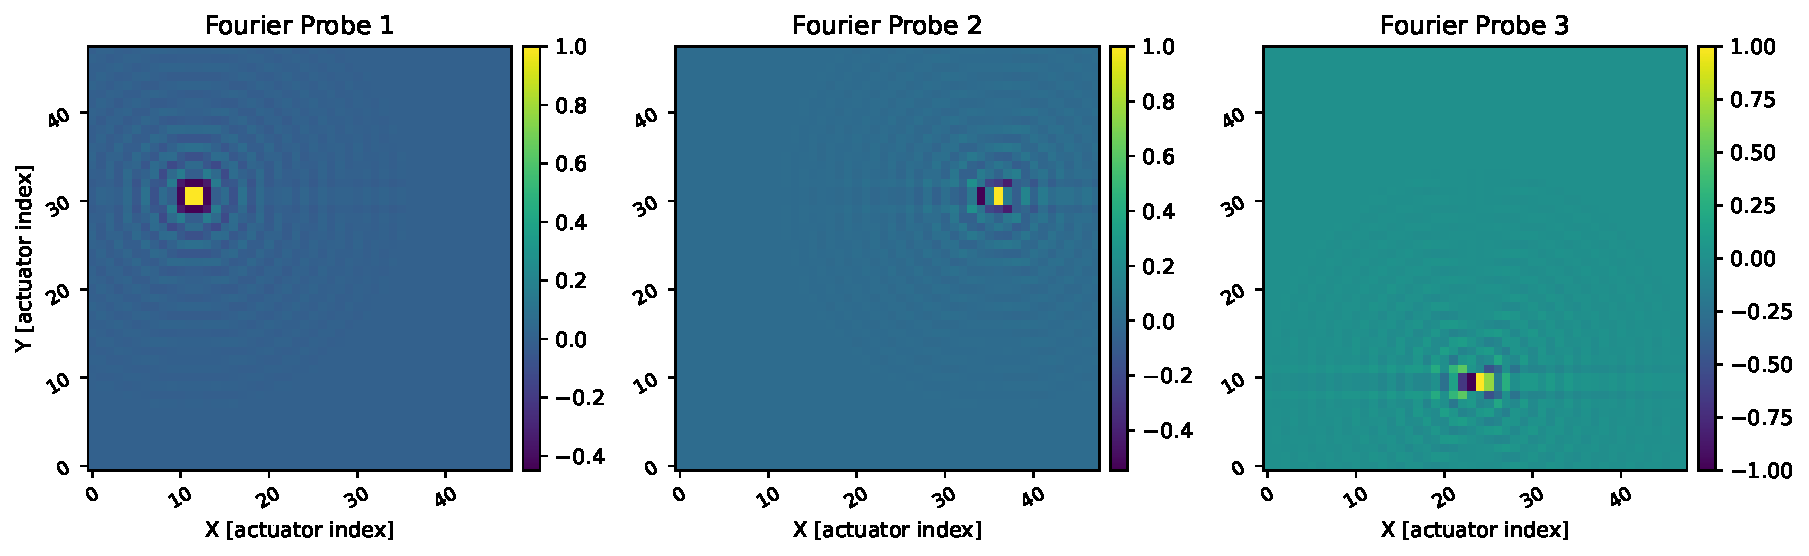
\includegraphics[scale=0.375]{figs-spc-band4b/fourier_probes.pdf}}
    \raisebox{-0.5\height}{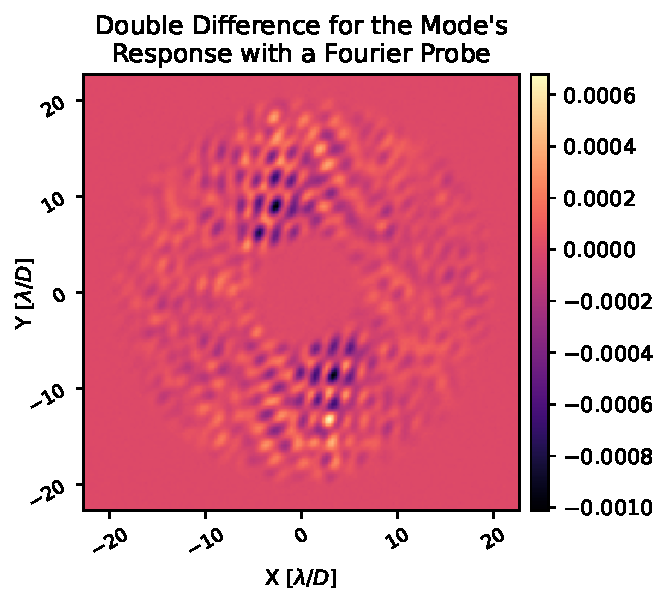
\includegraphics[scale=0.375]{figs-spc-band4b/dd_for_fourier_probe.pdf}}
    % \raisebox{-0.48\height}{\includegraphics[scale=0.275]{figs-spc-band4b/had_modes_3fourier_responses.png}}
    \caption{Here, the first three images are the Fourier probes for which the difference images are measured. To the far right is double difference response for the same example Hadamard mode using the first Fourier probe. As expected, the amplitude of the response using the Fourier probe is greater than with the single actuator probe, which helps mitigate the effects of noise.}
    \label{fig:spc-band4b-fourier-probe-examples}
\end{figure}

Using the Jacobian generated with Fourier probes, iEFC is tested again with the final solution portrayed in Figure \ref{fig:spc-band4b-fourier-modes}. Here, the final contrast is $1.41\times10^{-8}$. Because the final contrast was improved with the Fourier probes, the final exposure time had to be increased to 2400s, or 40min. Given the initial exposure time is 2s and the contrast is improved by about 3 orders of magnitude over the course of iEFC, the increase in exposure time is reasonable given the assumptions that have been made. In addition, the probe amplitude used within the controller was reduced from 25nm to 5nm over the course of the iterations. While this result remains about an order magnitude worse than what was obtained in the noiseless monochromatic simulation, the result is significantly better than with single actuator probes with a final contrast of $1.41\times10^{-8}$. 

\begin{figure}[h]
    \centering
    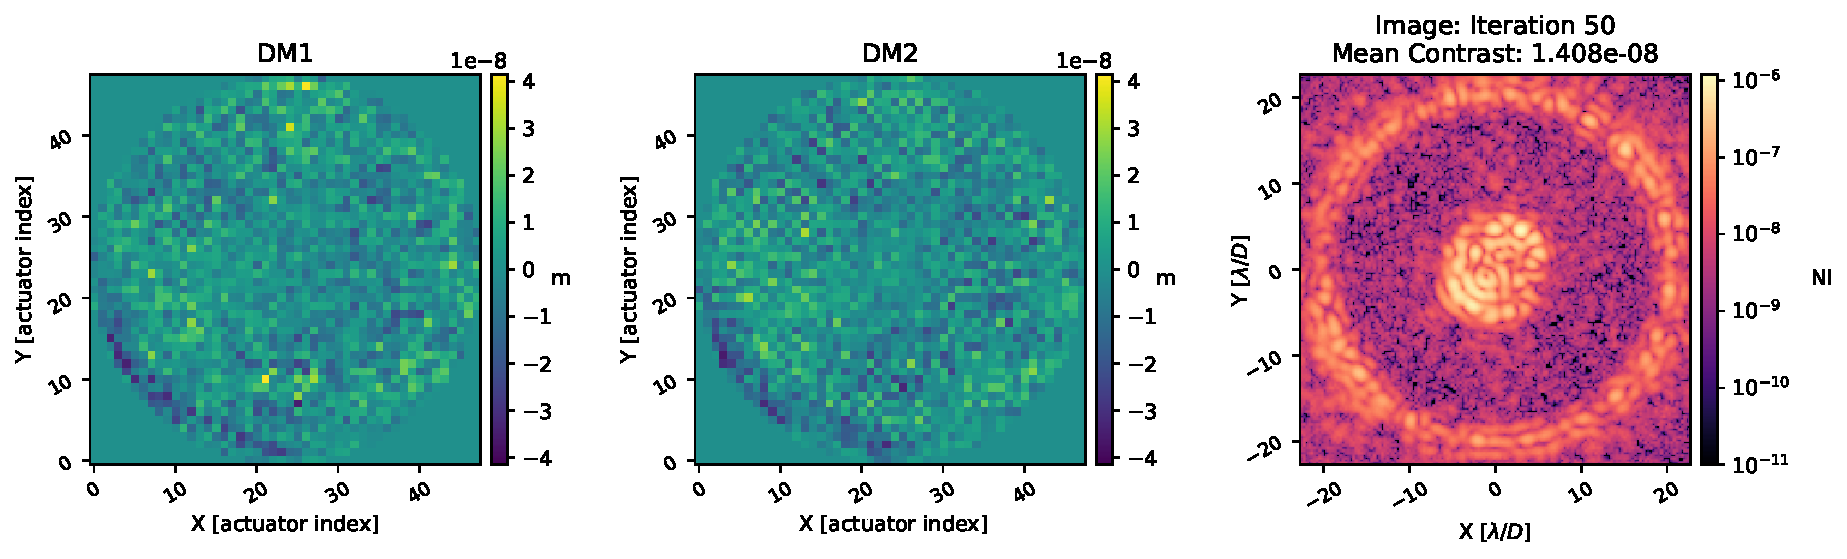
\includegraphics[scale=0.5]{figs-spc-band4b/had_modes_3fourier.pdf}
    \caption{The final DM solutions using the Fourier probes yielded a contrast of $1.41\times10^{-8}$. While not equivalent to the ideal monochromatic contrast, this fulfills the contrast requirement of the Coronagraph and demonstrates that the improved choice of probes can make iEFC a valid method for Roman.}
    \label{fig:spc-band4b-fourier-modes}
\end{figure}

This demonstration of iEFC with noise shows that the method is at least capable of yielding a dark hole on the order of $10^{-8}$ in the presence of a considerable amount of read noise and no gain. Significantly, the Hadamard modes with weighted Fourier probes are the best combination found here. More work is being done to obtain similar results using two probes as this would be ideal for reducing calibration times; however, three probes remain the best option for annular dark holes. Further testing using increased probe or calibration amplitudes could also reduce the exposure times required during calibration, but the nonlinearity of the DM response will become a greater issue in this case. In addition, simulations using EM gain can potentially reduce the required exposure times significantly, so this will be studied using a more accurate detector model by integrating the emccd\_detect package included within CGISim\footnote{\href{https://sourceforge.net/projects/cgisim/}{https://sourceforge.net/projects/cgisim/}} into iEFC simulations. 

\section{Conclusion}
\label{sec:conclusion}
The iEFC algorithm is an exciting method for the high-contrast imaging community. Like EFC, iEFC is naturally extended to coronagraphs with two DMs and capable of digging annular dark holes. This makes iEFC a potential method for the Roman Coronagraph, particularly for the SPC modes due to the minimal relinearization/recomputation required of the Jacobian. The simulations of iEFC for the SPC-WFOV mode demonstrate that contrasts on the order of $2\times10^{-9}$ can be achieved in the ideal monochromatic scenario. Significantly, iEFC can mitigate the risk of minor misalignments and faulty characterization of space-borne instruments as iEFC was demonstrated to perform well in the presence of a perturbation to the SPM. 

Hadamard modes are shown to be the ideal choice of modes for the SPC-WFOV as the controller converged the most rapidly. While the a calibration using three probes is estimated to take 27hours for a single narrow-band filter, further investigations will be done to truncate the number of modes such that the final contrast and convergence are not impacted, but calibration times can be reduced. In addition, more accurate modeling of the EMCCD with gain has the potential to reduce the estimated exposure times assumed for the results here. Nevertheless, the simulations with noise demonstrate that iEFC will be suitable to achieving the $10^{-7}$ contrast goal of the Roman Coronagraph. 

For a potential HWO instrument, iEFC is likely more suitable due to the larger aperture for photon collection. In particular, smaller dark holes such as that presented with the SVC simulation can require far fewer modes to be calibrated. Given the more challenging contrast goal of $10^{-10}$ for a HWO, a model-based HOWFSC algorithm will require a well characterized instrument with minimal model errors whereas iEFC can potentially be used to circumvent the necessity of a model. For this order of contrast requirements, additional investigations will be needed that include jitter and telescope instability during the calibration of the instrument. 

\subsection*{Acknowledgments}
Portions of this research were supported by funding from the Technology Research Initiative Fund (TRIF) of the Arizona Board of Regents and by generous anonymous philanthropic donations to the Steward Observatory of the College of Science at the University of Arizona. 

%\software{
This research made use of community-developed core Python packages, including: POPPY\cite{perrin-poppy-2017}, Astropy \cite{the_astropy_collaboration_astropy_2013}, Matplotlib \cite{hunter_matplotlib_2007}, SciPy \cite{jones_scipy_2001}, and
the IPython Interactive Computing architecture \cite{perez_ipython_2007}.
%}

Lastly, A.J. Riggs, Jaren Ashcraft, Kevin Derby, Aaron Goldtooth, and Ranger Maxwell have contributed through helpful discussions regarding simulations and wavefront control throughout the span of this research. 

\section{Code, Data, and Materials Availability}

All the code for simulations is made available through public repositories. The repository containing the end-to-end diffraction model constructed with POPPY can be found on Zenodo at \href{https://zenodo.org/record/8302380}{https://zenodo.org/record/8302380}\cite{milani-cgi-phasec-poppy}. Similarly, the repository containing the simulation material can be found at \href{https://zenodo.org/records/8302359}{https://zenodo.org/records/8302359}\cite{milani-roman-cgi-iefc}. 

The associated data that is required for the diffraction model along with the data obtained using iEFC can be found at \href{https://github.com/kian1377/cgi_phasec_poppy_data}{https://github.com/kian1377/cgi\_phasec\_poppy\_data}. 

%%%%% References %%%%%
\bibliography{report}   % bibliography data in report.bib
\bibliographystyle{spiejour}   % makes bibtex use spiejour.bst

%%%%% Biographies of authors %%%%%
\vspace{2ex}\noindent\textbf{Kian Milani} received his BS in Optical Engineering from the Wyant College of Optical Sciences in 2020. Now a PhD candidate in the same college, his work focuses on physical optics simulations and wavefront control techniques for coronagraphic instruments. 

\vspace{1ex}
\noindent Biographies and photographs of the other authors are not available.

\listoffigures
\listoftables

\end{spacing}
\end{document}



